\documentclass{beamer}

\mode<presentation>
{
  \usetheme{default}      
  \usecolortheme{beaver}
  \usefonttheme{professionalfonts}  
  \setbeamertemplate{navigation symbols}{}
  \setbeamertemplate{caption}[numbered]
  \setbeamertemplate{footline}[frame number]
} 
\usepackage{tikz}
\usepackage[english]{babel}
\usepackage[utf8]{inputenc}
\usepackage{graphicx}
\usepackage{booktabs} % For formal tables
\usepackage{times}
\usepackage{textcomp}
\usepackage{amsmath}
\usepackage{multirow}
\usepackage{algorithmic}
\usepackage{algorithm}

\usepackage{graphicx}
\usepackage{ragged2e}
 %\apptocmd{\frame}{}{\justifying}{} % Allow optional arguments after frame.0
\renewcommand{\raggedright}{\justifying}
%\newtheorem{mydef}{Definition}
\newtheorem{myteo}{Theorem}
\newtheorem{mycor}{Corollary}
\newtheorem{mylemma}{Lemma}
\renewcommand{\footnotesize}{\tiny}
%\renewcommand{\footnotesize}{\scriptsize}

\usepackage{multirow}

\usepackage[style=verbose]{biblatex}
\bibliography{biblio}


\renewcommand{\raggedright}{\justifying}

\newcommand{\HV}{{\sc hv}}

\usepackage{tcolorbox}
\tcbuselibrary{theorems}

\newtcbtheorem[number within=section]{mytheo}{Theorem}%
{colback=green!5,colframe=red!35!gray,fonttitle=\bfseries}{th}


\newtcbtheorem[number within=section]{mydef}{Definition}%
{colback=green!5,colframe=red!35!gray,fonttitle=\bfseries}{th}

\titlegraphic{
   
\includegraphics[width=3cm]{cimat.eps}\hspace*{1.75cm}~%
   
\includegraphics[width=3cm]{CONACYT.eps}
}

\title[Your Short Title]{Optimización Evolutiva Multi-objetivo}
\author{\textcolor{red}{Dr. Carlos Segura González} \\ Joel Chacón Castillo}
\institute{Centro de Investigación de Matemáticas}

%\date{November 07, 2019}

\begin{document}

\begin{frame}
  \titlepage
\end{frame}

%\begin{frame}{Outline}
%\begin{itemize}
%\item Introduction
%\item Maximum Likelihood Estimate
%\item Proposal
%\item MIX-SQP Algorithm
%\item Experimental Validation
%\item Conclusions
%\end{itemize}
%\end{frame}
\begin{frame}{Esquema General}
\frametitle{Esquema General}
\tableofcontents
\end{frame}


\section{Introducción y antecedentes}



\begin{frame}{Optimizadores estocásticos poblacionales}
    \begin{itemize}
    \scriptsize
    \justifying
        \item Una meta-heurística es un proceso maestro que de forma iterativa guía y modifica un conjunto de operaciones heurísticas con el fin de producir soluciones de calidad de forma eficiente \footcite{voss2012meta}.
        \item Las meta-heurísticas poblacionales consideran múltiples soluciones en cada iteración.
        \item Algunas meta-heurísticas poblacionales más populares son las siguientes:
        \begin{itemize}
        \scriptsize
            \item Algoritmos genéticos (GA).
            \item Programación genética (GP).
            \item Programación evolutiva (EP).
            \item Evolución diferencial (DE).
            \item Estrategia evolutiva (ES).
            \item Algoritmos de estimación de distribución (EDA).
            \item Optimización por enjambre de particulas (PSO).
            \item Algoritmos de optimización por colonias de hormigas (ACO).
        \end{itemize}{}
    \end{itemize}{}
\end{frame}{}


\begin{frame}{Optimizadores estocásticos poblacionales}

\begin{figure}[H]
\centering
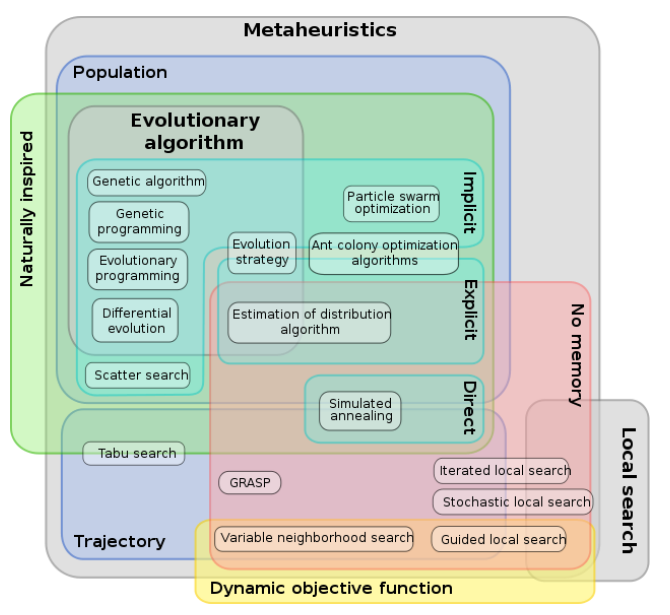
\includegraphics[width=0.6\textwidth]{clasificacion.png}
\caption{Clasificación de las meta-heurísticas más populares\footcite{beheshti2013review}.}
\label{fig:clasificacion}
\end{figure}
\end{frame}

\begin{frame}{Problemas de las meta-heurísticas poblacionales}
\begin{itemize}
 \scriptsize
    \item La mayoría de las meta-heurísticas poblacionales tienen problemas de convergencia, y no es fácil controlar la velocidad en que convergen.
   % \item Una de las fallas más típicas es la convergencia prematura.
%    \item La convergencia prematura es cuando los %miembros de la población son `atrapados' en ciertas regiones del espacio de búsqueda.
    \item Se dice que un algoritmo converge de forma prematura cuando mucho antes de alcanzar el criterio de paro, todas las soluciones están en una zona muy pequeña del espacio de búsqueda\footcite{Crepinsek:13}.
    
\begin{figure}[H]
\centering
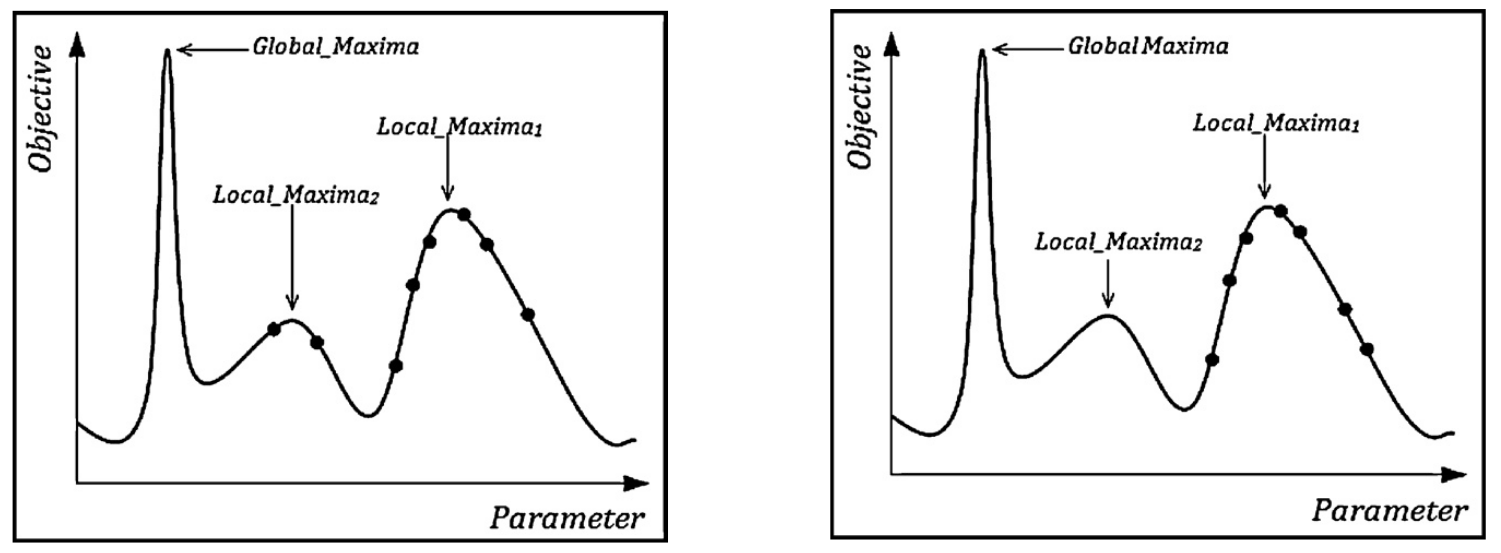
\includegraphics[width=0.7\textwidth]{landscape.png}
\caption{\scriptsize Escenarios de convergencia de una meta-heurística poblacional\footcite{alam2012diversity}.}
\label{fig:clasificacion}
\end{figure}
\end{itemize}
\end{frame}

\begin{frame}{Algoritmos Evolutivos (EAs)}
    \begin{itemize}
       \item Son un tipo de meta-heurísticas poblacionales.
        \item Son un enfoque ampliamente utilizado para resolver distintos tipos de problemas de optimización.
        
        \item Se han desarrollado diversas variantes que han sido aplicadas en múltiples campos, como en transporte, economía e ingeniería\footcite{dasgupta2013evolutionary}.
        
        \item Los EAs pueden ser aplicados en problemas de dominio continuo y/o de dominio discreto.
        
        \item Este tipo de algoritmos han sido exitosos principalmente en problemas del tipo NP-completo cuya solución exacta no es conocida.
    \end{itemize}{}
\end{frame}

\begin{frame}{Esquemas de los algoritmos evolutivos}
  \begin{algorithm}[H]
  \begin{scriptsize}
%\algsetup{linenosize=\tiny}
\caption{Evolutionary Algorithm} 
\begin{algorithmic}[1]
 	\STATE \textbf{Initialization}: Generate an initial population $P_0$ with $N$ individuals.
	\STATE \textbf{Evaluation}: Evaluate all individuals in the population.
	\STATE Assign $t=0$
	\WHILE{(not stopping criterion)}
	   \STATE \textbf{Mating selection}: Fill the mating pool performing selection on $P_t$.
	   \STATE \textbf{Variation}: Apply crossover and mutation operators to the mating pool to create an offspring population $Q_t$ with $N$ individuals.
		 \STATE \textbf{Evaluation}: Evaluate all individuals in $Q_t$.
	   \STATE \textbf{Survivor selection}: Generate $P_{t+1}$ by applying the replacement operator using $P_t$ and $Q_t$.
	   \STATE $t=t+1$
	\ENDWHILE
	\end{algorithmic}

\end{scriptsize}
\end{algorithm}
\end{frame}

\begin{frame}{Principios de diseño de un algoritmo poblacional}
\begin{itemize}
\justifying
    \item Como parte del diseño de una meta-heurística poblacional, para tratar adecuadamente la convergencia debería existir un balanceo entre \underline{exploración} e \underline{intensificación} del espacio de búsqueda \footcite{herrera1996adaptation}.
    \item La exploración del espacio de búsqueda evalúa regiones que no han sido muestreadas con el fin de detectar regiones promisorias.
    \item La intensificación realiza una búsqueda más profunda con el fin de encontrar soluciones de mayor calidad.
    
\end{itemize}
\begin{figure}
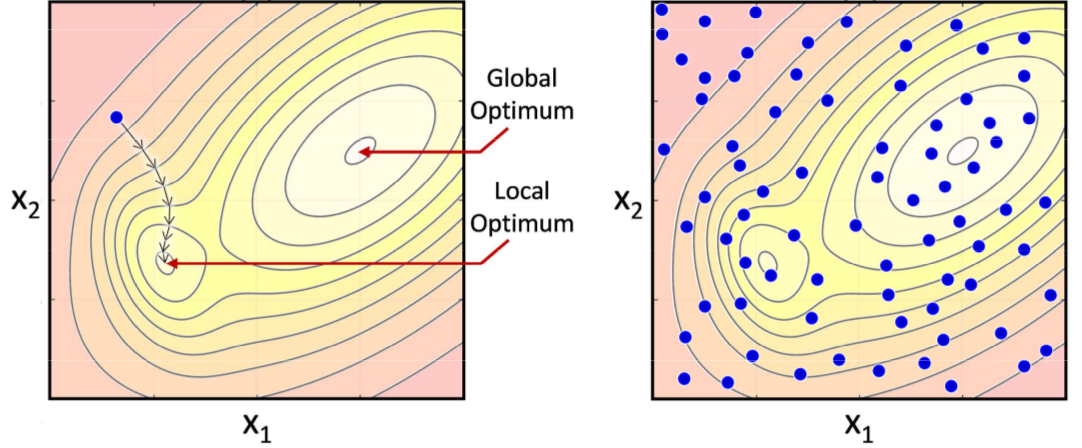
\includegraphics[width=0.6\textwidth]{exploration_2.png}
%\caption{Clasificación de las Meta-heurísticas más populares\footcite{beheshti2013review}.}
\label{fig:clasificacion}
\end{figure}

\end{frame}

\begin{frame}{¿Cómo tratar la convergencia?}
\begin{itemize}
\justifying
    \item Una grado de exploración elevado puede causar una falta de intensificación en las regiones más prometedoras (\textbf{alta diversidad}).
    \item Por otra parte, una intensificación elevada provoca una pérdida de \textbf{diversidad} en la población.
    \item ¿Cómo fomentar este balanceo en una meta-heurística poblacional? (línea de investigación activa).
\end{itemize}
\end{frame}

\begin{frame}{¿Cómo tratar la convergencia?}
\begin{itemize}
\justifying
    \item Algunas técnicas controlan de manera directa o indirecta la cantidad de diversidad mantenida por el algoritmo\footcite{Crepinsek:13}.
    \item Éstas técnicas son identificadas de forma general como enfoques uni-proceso y multi-proceso.
    \item Una taxonomía ampliamente utilizada de las estrategias para promover la diveridad son:
    \begin{itemize}
        \item Enfoques basados en la selección \footcite{eiben2003introduction}.
        \item Enfoques basados en población\footcite{alba2005parallel}.
        \item Enfoques basados en la cruza y/o la mutación\footcite{yu2014differential}.
    \end{itemize}
\end{itemize}
\end{frame}


\begin{frame}{Esquemas de reemplazamiento basados en diversidad}
\begin{itemize}
    \item Los esquemas de reemplazamiento se utilizan para diversificar a los individuos sobrevivientes, de forma que los operadores de reproducción puedan generar nuevas soluciones en diferentes regiones \footcite{eiben1998evolutionary}.
    \item Existen varias estrategias de reemplazo para forzar la diversidad en la población, algúnas populares son:
    \begin{itemize}
    \scriptsize
       \item \textit{Restricted Tournament Selection} - RTS (\citeyear{harik1995finding}) por \citeauthor{harik1995finding}.
       \item \textit{Contribution of Diversity and Replacement of the Worst} - CD/RW (\citeyear{lozano2008replacement}) por \citeauthor{lozano2008replacement}.
       \item \textit{Hybrid Genetic Search with Adaptive Diversity Control} - HGSADC (\citeyear{vidal2013hybrid}) por \citeauthor{vidal2013hybrid}.
       \item \textit{Multi-dynamic} (\citeyear{segura2016novel}) por \citeauthor{segura2016novel}. 
       \item \textit{Best-Non Penalized} (\citeyear{romero2018memetic}) por \citeauthor{romero2018memetic}.
    \end{itemize}
\end{itemize}
\end{frame}

\section{Conceptos}

\begin{frame}{Definición de un problema mono-objetivo}
    \begin{itemize}
\justifying
\item Un problema de optimización mono-objetivo puede ser definido de la siguiente forma\footcite{nocedal2006numerical}:
%
\end{itemize}
\begin{equation}
\scriptsize
\begin{split}
Minimizar/Maximizar \quad &f(x)  \\
sujeto\quad a \quad  &g_j(x) \geq 0 \quad j = 1,2, ... J\\
&h_k(x) = 0, \quad k=1,2, ..., K\\
&x_i^{(L)} \leq x_i \leq x_i^{(U)} \quad i = 1,2, ..., n 
\end{split}
\label{eqn:MOOP}
\end{equation}
donde $x_i^{(L)}, x_i^{(U)}$ son el límite inferior y superior de la $i$-ésima variable, $g_j(x)$ y $h_k(x)$ son restricciones de desigualdad e igualdad respectivamente.
%
%\begin{itemize}
%    \item Si el problema tiene dominio continuo $x \in \Re^n$.
%\end{itemize}
\end{frame}



\begin{frame}{Definición de un problema multi-objetivo}
\begin{itemize}
    \item Un problema de optimización multi-objetivo tiene un número de funciones objetivo en conflicto las cuales se deben minimizar o maximizar.
    \item Similarmente a un problema de optimización mono-objetivo, un problema multi-objetivo tiene un número de restricciones que cualquier solución factible debería satisfacer.
\end{itemize}

La forma general de un problema multi-objetivo se puede definir de la siguiente forma\footcite{Joel:Kalyanmoy}:
\begin{equation}
\scriptsize
\begin{split}
Minimizar/Maximizar \quad &f_m(x), \quad m=1,2,...,M  \\
sujeto\quad a \quad  &g_j(x) \geq 0 \quad j = 1,2, ... J\\
&h_k(x) = 0, \quad k=1,2, ..., K\\
&x_i^{(L)} \leq x_i \leq x_i^{(U)} \quad i = 1,2, ..., n 
\end{split}
\label{eqn:MOOP}
\end{equation}
\end{frame}



\begin{frame}{Definición de dominancia}
\justifying
\begin{itemize}
\justifying
    \item A diferencia del caso mono-objetivo, en el ámbito multi-objetivo no es posible comparar de forma directa dos soluciones $x, y \in \Omega$.
    \item Una alternativa para comparar soluciones es considerando la relación de dominancia.
\end{itemize}
\begin{mydef}{Dominancia}{}
\scriptsize
Se dice que una solución $x$ domina a otra solución $y$ ($x \prec y$), si se cumplen las siguientes dos condiciones:
    \begin{itemize}
        \item La solución $x$ no es peor que la solución $y$ en ninguno de los objetivos.\\
$\forall m \in \{ 1, 2, ..., M \}: f_m(x) \leq f_m(y)$
\justifying
        \item La solución $x$ es estrictamente mejor que la solución $y$ en al menos un objetivo.\\
$\exists m \in \{ 1, 2, ..., M \}: f_m(x) < f_m(y)$
    \end{itemize}
\end{mydef}
\end{frame}

\begin{frame}{Dominancia}
\begin{figure}[H]
\centering
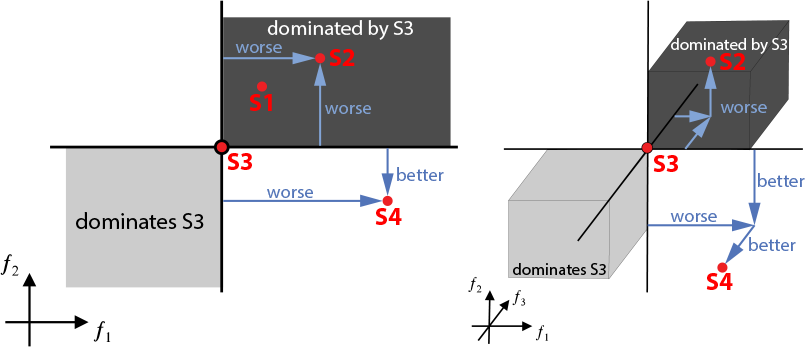
\includegraphics[width=0.9\textwidth]{dominance_scheme.png}
\caption{\scriptsize Esquema de dominancia en dos y tres objetivos respectivamente\footcite{WinNT}.}
\end{figure}
\end{frame}

\begin{frame}{Conceptos multi-objetivo}

\begin{mydef}{Conjunto no dominado}{}
\scriptsize
    Es la colección de todas la soluciones incomparables y no dominadas relacionadas al conjunto $S \subseteq \Omega$ .
    \begin{equation*}
        NDS(S) = \{ s \in S: \nexists s\prime \in S, s\prime \prec s \}
    \end{equation*}
\end{mydef}

\begin{mydef}{Conjunto Óptimo de Pareto}{}
\scriptsize
%\begin{itemize}
%    \item 
Es un conjunto de vectores de decisión óptimos no dominados en $\Omega$.
       \begin{equation*}
        POS = \{ x^* \in \Omega : \nexists x \in \Omega \subset \Re^n, x \prec x^*  \}
    \end{equation*}
%\end{itemize}{}
\end{mydef}

\begin{mydef}{Frente de Pareto}{}
\scriptsize
%\begin{itemize}
    %\item 
    La imágen del conjunto óptimo de Pareto es el frente de Pareto óptimo. 
        \begin{equation*}
             POF = \{ f(x^*) \in Z \subset \Re^m: x^* \in POS \} 
        \end{equation*}
%\end{itemize}{}
\end{mydef}

%\begin{figure}[H]
%\centering
%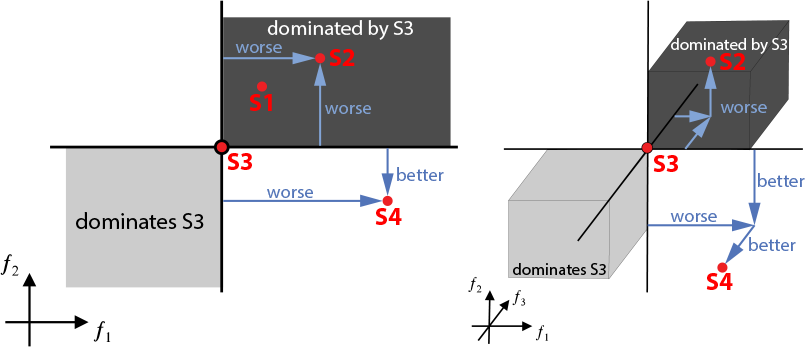
\includegraphics[width=0.8\textwidth]{dominance_scheme.png}
%\caption{\scriptsize Definición de dominancia con dos y tres objetivos respectivamente\footcite{WinNT}.}
%\end{figure}
\end{frame}


\begin{frame}{Conceptos multi-objetivo}

\begin{figure}[H]
\centering
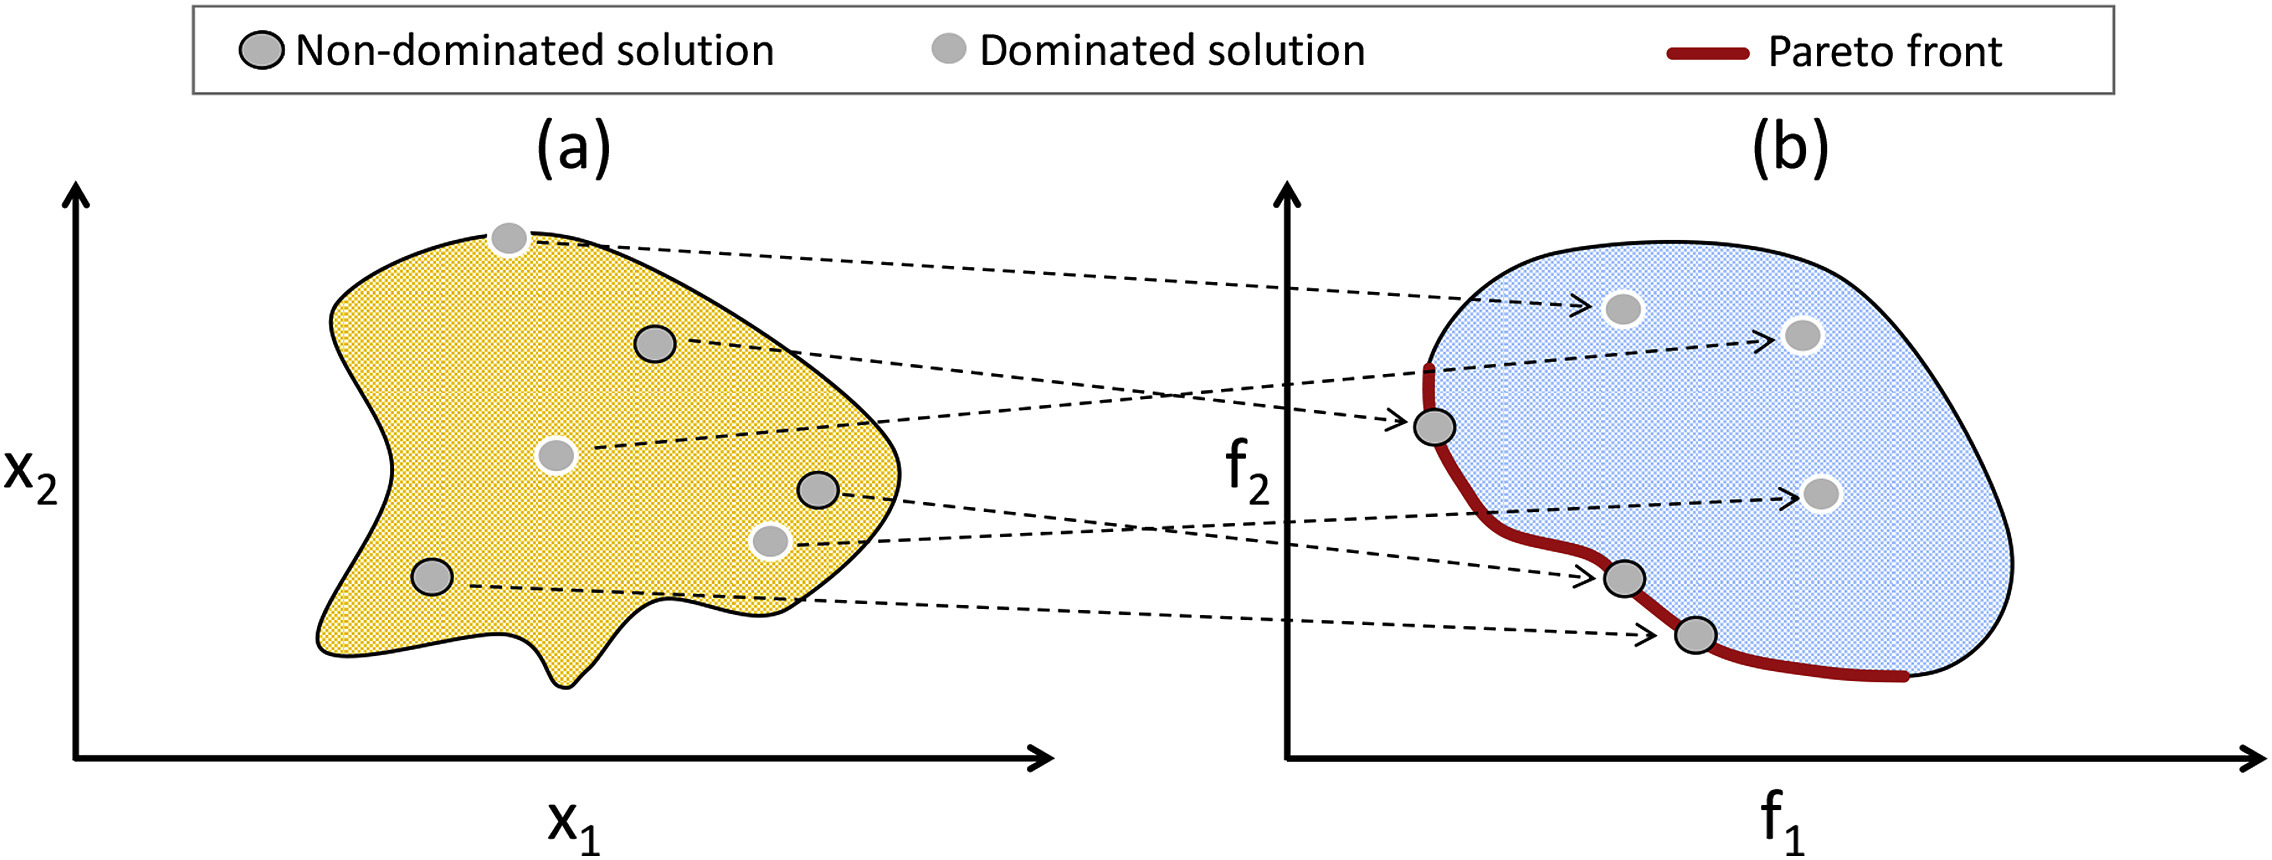
\includegraphics[width=0.9\textwidth]{Mapping.jpg}
\caption{\scriptsize Mapeo del espacio de las variables (a) en el espacio objetivo (b)\footcite{alam2012diversity}.}
\end{figure}
\end{frame}




\section{Clasificación de algoritmos multi-objetivo}

\begin{frame}{Paradigmas de los algoritmos multi-objetivo}
Una clasificación muy aceptada de los MOEAs es\footcite{trivedi2016survey}:
\begin{itemize}
\justifying
\item \textbf{Basados en dominancia}.
   \begin{itemize}
       \item Utilizan la relación de dominancia de Pareto.
   \end{itemize}
\justifying
\item \textbf{Basados en descomposición}.
\begin{itemize}
       \item Transforman un problema multi-objetivo en un conjunto de problemas de optimización mono-objetivo que son resueltos simultáneamente.
   \end{itemize}
\justifying
\item \textbf{Basados en indicadores}.
    \begin{itemize}
        \item Combinan el grado de convergencia y/o la diversidad del espacio objetivo con una métrica.
    \end{itemize}
\end{itemize}

\justifying
\scriptsize
Actualmente no existe un algoritmo el cual sea considerado superior, por lo tanto usualmente se selecciona al menos un algoritmo de cada tipo como parte del estado del arte.
\end{frame}





\begin{frame}{Algoritmos basados en dominancia}
Algunos de los algoritmos multi-objetivo clásicos que son basados en dominancia:
\begin{itemize}
\scriptsize
    %\item  Algoritmo Genético Basado en Ordenación de No Dominados II (\textit{Non-dominated Sorting Genetic Algorithm II} - NSGA-II)\footcite{Joel:NSGAII}.
    \item \citeyear{Joel:MOGA}, \textit{Multi-objective Genetic Algorithm} (MOGA), \\ \citeauthor{Joel:MOGA}.
    \item \citeyear{Joel:NPGA}, \textit{Niche Pareto Genetic Algorithm} (NPGA), \\ \citeauthor{Joel:NPGA}.
    \item \citeyear{zitzler2001spea2}, \textit{Strength Pareto Evolutionary Algorithm} (SPEA2), \\ \citeauthor{zitzler2001spea2}.
    \item \citeyear{Joel:NSGAII},  \textbf{\textit{Non-dominated Sorting Genetic Algorithm II} (NSGA-II)}, \\ \citeauthor{Joel:NSGAII}.
    \item \citeyear{Joel:GDE3}, \textit{Generalized Differential Evolution} (GDE3), \\ \citeauthor{Joel:GDE3}.
\end{itemize}
\end{frame}


\begin{frame}{Non-dominated Sorting Genetic Algorithm II (NSGA-II)}
\begin{itemize}
\scriptsize
\item Es uno de los primeros algoritmos multi-objetivo que introducen elitismo.
\item Realiza una clasificación por frentes de baja complejidad $O(MN^2)$, estrategia ampliamente utilizada en multi-objetivo conocida como \textit{fast-non-dominated-sortig} (convergencia al frente de Pareto).
\item Considera un operador de amontonamiento o \textit{crowding} (diversidad en el frente de Pareto).
\begin{equation*}
   d_i = \sum_{j=1}^m \frac{f_j^{i+1} - f_j^{i-1}   }{f_j^{max} - f_j^{min}}
\end{equation*}
\end{itemize}

\begin{figure}[H]
\centering
\begin{tabular}{c c}
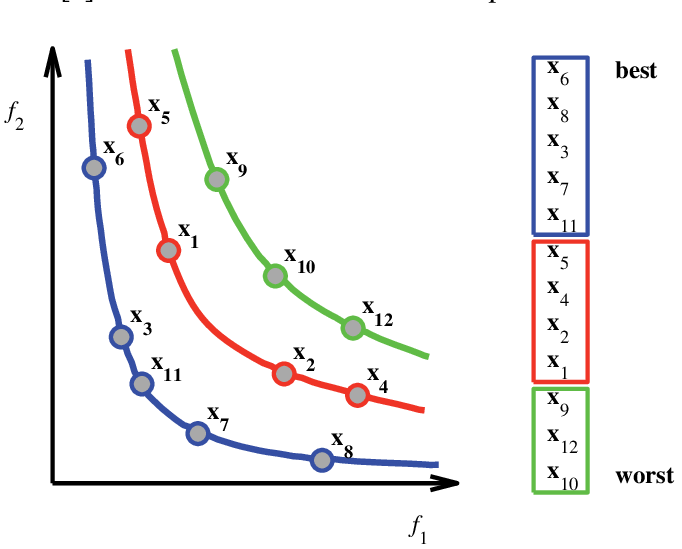
\includegraphics[width=0.3\textwidth]{fronts.png} & 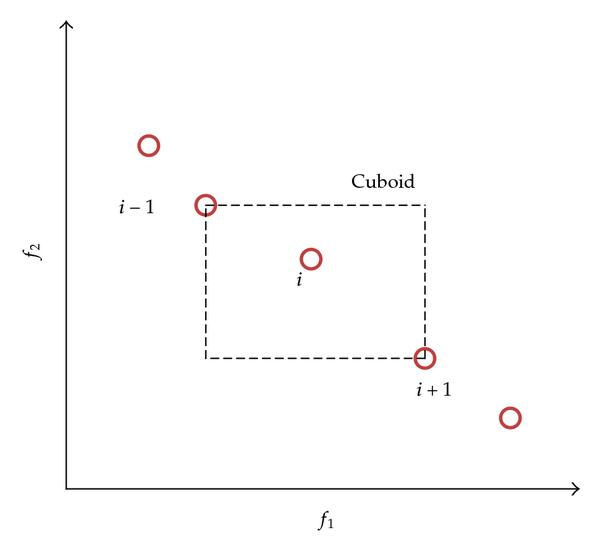
\includegraphics[width=0.3\textwidth]{crowding_nsgaii.jpg} 
\end{tabular}
\caption{\scriptsize Clasificación por frentes (izquierda) y distancia de crowding (derecha)\footcite{kadlec2016multi}.}
\end{figure}
\end{frame}


\begin{frame}{Non-dominated Sorting Genetic Algorithm II (NSGA-II)}
\begin{itemize}
\scriptsize
\item Incorpora el operador de cruza SBX y el operador de mutación polinomial.
%\item 
%\item Es uno de los primeros algoritmos multi-objetivo que introducen elitismo.
%\item Realiza una clasificación por frentes de baja complejidad $O(MN^2)$, estrategia ampliamente utilizada en multi-objetivo conocida como \textit{fast-non-dominated-sortig}.
%\item Considera un operador de amontonamiento o \textit{crowding}. 
\end{itemize}

\begin{figure}[H]
\centering
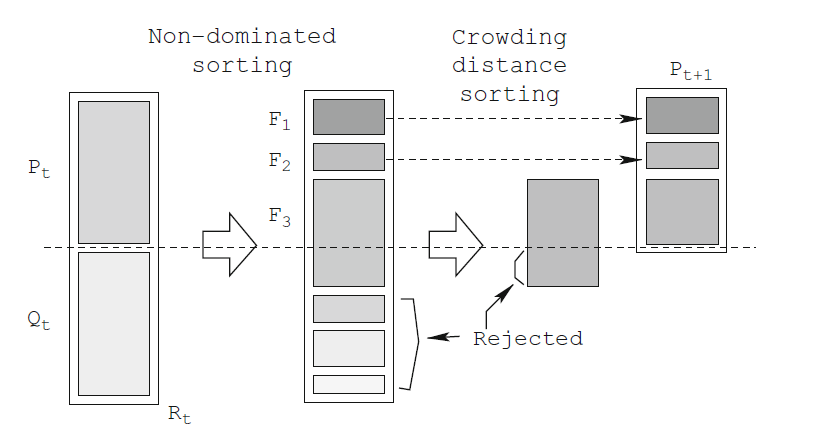
\includegraphics[width=0.8\textwidth]{nsgaii_main.png}
\caption{\scriptsize Procedimiento principal del NSGA-II\footcite{Joel:NSGAII}.}
\end{figure}
\end{frame}

 
\begin{frame}{Algoritmos basado en descomposición}
Algunos de los algoritmos multi-objetivo clásicos que son basados en descomposición son:
\begin{itemize}
     \scriptsize
    \item \citeyear{ishibuchi1998multi}, \textit{Multi-objective Genetic Local Search Algorithm} (MOGLS), \\ \citeauthor{ishibuchi1998multi}.
    \item \citeyear{murata2002cellular}, \textit{Cellular Multi-objective Genetic Algorithm} (C-MOGA), \\ \citeauthor{murata2002cellular}.
    \item \citeyear{Joel:MOEAD}, \textbf{\textit{Multi-objective Evolutionary Algorithm based in Decomposition} (MOEA/D)}, \\ \citeauthor{Joel:MOEAD}.
     \item \citeyear{li2009multiobjective}, \textit{Multi-objective Evolutionary Algorithm based in Decomposition with DE}, (MOEA/D -CEC 2009), \\ \citeauthor{li2009multiobjective}.
    \item \citeyear{Joel:MOEAD_AMS}, \textit{MOEA/D - Adaptive Mating Selection Mechanism} (MOEA/D - AMS), \\ \citeauthor{Joel:MOEAD_AMS}.
    \item \citeyear{zhou2015all}, \textit{MOEA/D - Generalized Resource Allocation} (MOEA/D-GRA), \\ \citeauthor{zhou2015all}.
\end{itemize}
\end{frame}

\begin{frame}{Multi-objective Evolutionary Algorithm based in Decomposition (MOEA/D)}
\scriptsize
%\item Realiza la descomposición de un problema de optimización multi-objetivo en un conjunto de subproblemas de optimización mono-objetivo de forma simultánea.
La versión original del MOEA/D\footcite{ishibuchi1998multi} tiene las siguientes particularidades:
\begin{itemize}
\scriptsize
    \item Cada subproblema está definido por un vector de pesos.
    \item Define vecindades de cada subproblema en relación a su ubicación en el espacio objetivo.
    \item Sólo se hacen emparejamientos y reemplazamientos en los vecindarios.
    \item Considera el operador de cruza SBX y el operador de mutación polinomial.
\end{itemize}
\begin{figure}[H]
\centering
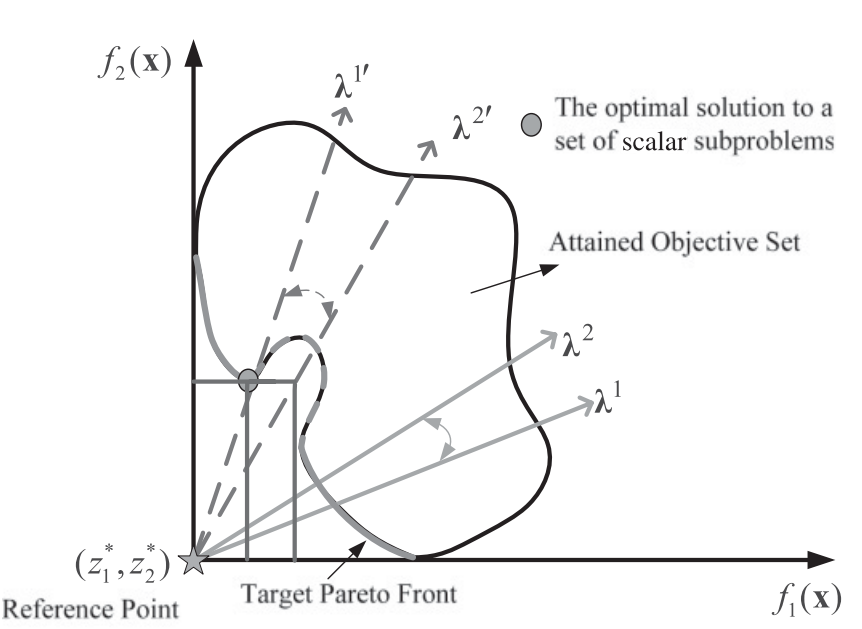
\includegraphics[width=0.35\textwidth]{moead_diagrama.png}
\caption{\scriptsize Vectores de pesos y su punto óptimo con el enfoque de Tchebysheff\footcite{Joel:MOEAD_Adaptative}}
\end{figure}

\end{frame}

\begin{frame}{Multi-objective Evolutionary Algorithm based in Decomposition (MOEA/D)}
%\begin{itemize}
\scriptsize
Una versión bastante popular y que tomó el primer lugar en la competancia del CEC 2009 (\textit{Congress on Evolutionary Computation}) es el  MOEA/D-DE que además considera las siguientes características\footcite{li2009multiobjective}: 
\begin{itemize}
\scriptsize
    \item Reestricciones de emparejamiento y de reemplazamiento.
    \item Para mantener diversidad en el espacio de las variables se considera emparejamiento en toda la población con probabilidad $1 - \delta$ y en el vecindario con probabilidad $\delta$. 
    \item Implementa un mecanismo que administra las evaluaciones a función en cada subproblema mejor conocido como \textit{Dynamical Resource Allocation}.
    \item Utiliza operadores de evolución diferencial y el operador de mutación polinomial.
\end{itemize}
%\end{itemize}
\end{frame}



\begin{frame}{Funciones de utilidad}
\justifying
\scriptsize
Existe una gran variedad de funciones de utilidad para convertir un problema multi-objetivo en un conjunto de problemas de un sólo objetivo, algunos de los más utilizados son\footcite{raquel_2018}:
\begin{itemize}
\scriptsize
\item Suma ponderada (\textit{Weighted Sum})
\begin{equation*}
\min_{} g^{ws}(x | \lambda, z^*) = \sum_{i=1}^m \lambda_i f_i(x)     
\end{equation*}
\item Tchebysheff 
\begin{equation*}
    \min_{} g^{te}(x | \lambda, z^*) = \max_{1 \leq i \leq m } \{ \lambda_i | f_i(x) - z_i^* | \}
\end{equation*}{}
\item Función de escalarización alcanzado (\textit{Achieved Scalarized Function} - ASF)
\begin{equation*}
    \min_{} g^{te}(x | \lambda, z^*) = \max_{1 \leq i \leq m } \{ \frac{| f_i(x) - z_i^* |}{\lambda_i}\}
\end{equation*}{}
\item Intersección del límite de penalización (\textit{Penalty Boundary Intersection} - PBI)
\begin{equation*}
\begin{split}
    \min g^{bi}(x | \lambda, z^*) &= d_1 + \theta d_2    \\
    sujeto \quad  a \quad d_1 &= \frac{|| (F(x) - z^*)^T \lambda  || }{|| \lambda ||}, \quad d_2 = || F(x) - (z^* + d_1 \lambda )||
\end{split}
\end{equation*}
\end{itemize}
\end{frame}

\begin{frame}{Funciones de utilidad}
\begin{figure}[H]
\begin{tabular}{c c}
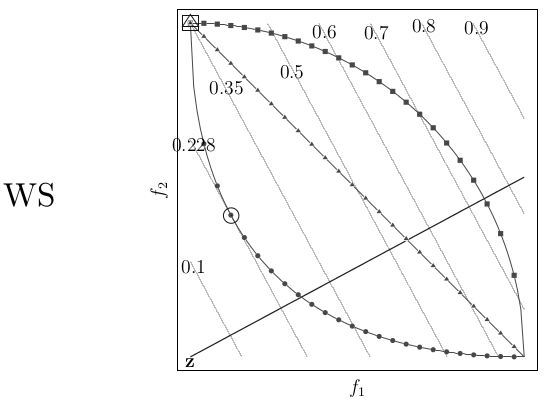
\includegraphics[width=0.4\textwidth]{ws.png}     &  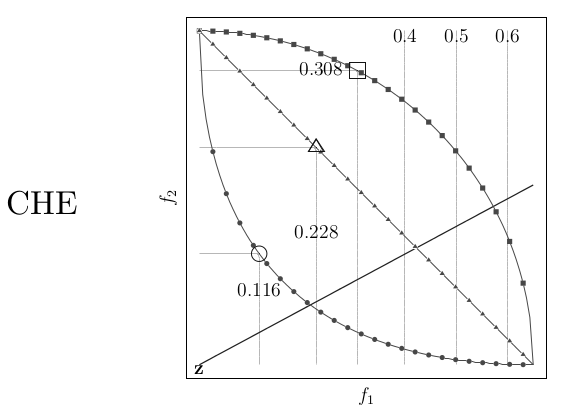
\includegraphics[width=0.42\textwidth]{che.png} \\
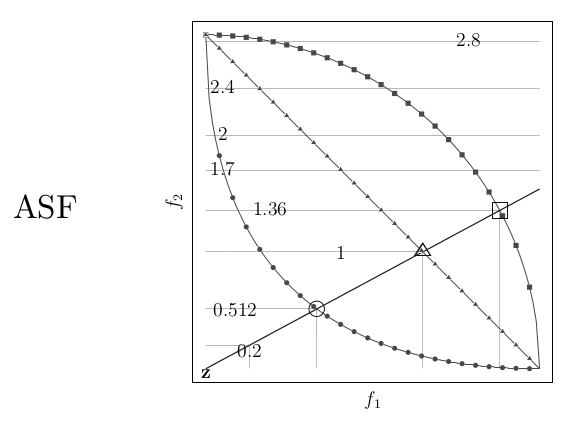
\includegraphics[width=0.4\textwidth]{asf.png}     &  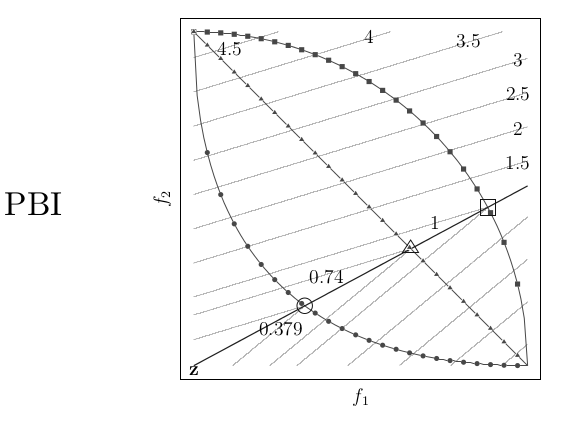
\includegraphics[width=0.4\textwidth]{pbi.png} \\
\end{tabular}
\centering
\caption{\scriptsize Mapa de contorno de las funciones de utilidad\footcite{raquel_2018}.}
\end{figure}
\end{frame}



\begin{frame}{Algoritmos basados en indicadores}
Algunos de los algoritmos clásicos multi-objetivo basados en indicadores son:
\begin{itemize}
\scriptsize
   \item \citeyear{Joel:IBEA}, \textit{Indicator Based-Selection Evolutionary Algorithm } (IBEA), \\ \citeauthor{Joel:IBEA}.
   \item \citeyear{Joel:SMSEMOA}, \textbf{\textit{S-Metric Selection Evolutionary Multi-objective Optimization Algorithm} (SMS-EMOA)}, \\ \citeauthor{Joel:SMSEMOA}.
   \item \citeyear{Joel:FV-MOEA}, \textit{Fast Hypervolume Multi-objective Evolutionary Algorithm} (FV-MOEA), \\ \citeauthor{Joel:FV-MOEA}.
   \item \citeyear{Joel:MOMBI-II}, \textit{Many-Objective Metaheuristic Based on $R2$ Indicador} (MOMBI-II), \\ \citeauthor{Joel:MOMBI-II}.
\end{itemize}
\end{frame}



\begin{frame}{S-Metric Selection Evolutionary Multi-objective Optimization Algorithm (SMS-EMOA)}
\begin{itemize}
\scriptsize
\item Implementa un operador de selección especial que combina la métrica de hipervolumen con el concepto de dominancia de Pareto.
%
\item Considera un esquema de selección de estado estable (\textit{Steady State}).
\item Una propuesta incorpora una clasificación por frentes y sólo considera el HV en el conjunto no dominado (primer frente).
\end{itemize}
\begin{figure}[H]
\centering
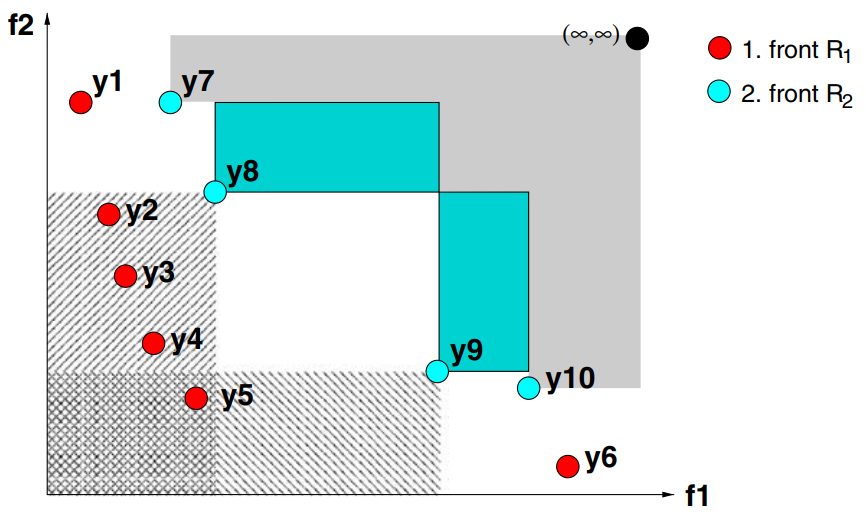
\includegraphics[width=0.5\textwidth]{sms_emoa.png}
\caption{\scriptsize Contribución del HV de cada solución\footcite{Joel:SMSEMOA}.}
\end{figure}
\end{frame}

\section{Análisis de resultados en multi-objetivo}

\begin{frame}{Análisis de los resultados}
Existen distintas herramientas para estimar la calidad de un conjunto de soluciones generadas por un optimizador, algunas de las mas utilizadas son las siguientes:
\begin{itemize}
\justifying
\item \textbf{Métricas de desempeño}
   \begin{itemize}
     \item La Distancia Generacional Invertida (IGD).
     \item La Distancia Generacional Invertida Modificada (IGD+).
     \item El hipervolumen (HV).
   \end{itemize}
\item \textbf{Análisis estadísticos}
  \begin{itemize}
      \item Pruebas estadísticas.
      \item Tabla general de las estadísticas.
  \end{itemize}
  \item \textbf{Superficies de cubrimiento}
\end{itemize}
\end{frame}

\begin{frame}{Métricas de desempeño}
   \begin{itemize}
	\scriptsize
        \item En optimización multi-objetivo se han propuesto varios indicadores o métricas para evaluar la calidad de un conjunto de soluciones.
	\item En general los indicadores son métricas que determinan el grado de convergencia al frente de Pareto y/o diversidad de las soluciones.
	\item El indicador más frecuente es el hipervolumen debido a que es el único del tipo \textit{Pareto compliant}\footcite
{Joel:ComparativeCaseStudy}.
	\item Ser \textit{Pareto compliant}\footcite{Joel:ComparacionMetricas} quiere decir que el indicador no contradice el orden inducido por la relación de dominancia.
	\begin{equation*}
	   A \succeq B \wedge  B \not \succeq A \rightarrow I(A) > I(B)
	\end{equation*}
   \end{itemize} 
\end{frame}


\begin{frame}{Hipervolumen}
\begin{itemize}
\scriptsize
\justifying
\item Es un indicador unario conocido como ``Pareto Compliant''\footcite{zitzler1999evolutionary}.
\item Este indicador determina la porción del espacio objetivo que es dominado por las soluciones de un conjunto $A$, el cual es limitado por un punto de referencia $r \in \Re^m$ indicado en la ecuación (\ref{eqn:HV}), donde $\Lambda$ denota la medición de Lebesgue y $r$ debería ser dominado por todos los elementos en $A$.
\end{itemize}
\begin{equation}\label{eqn:HV}
\scriptsize
    HV(A;r) = \Lambda \left (  \bigcup_{a \in A} \{ x | a \prec x \prec r \} \right )
\end{equation}

\begin{figure}[H]
\centering
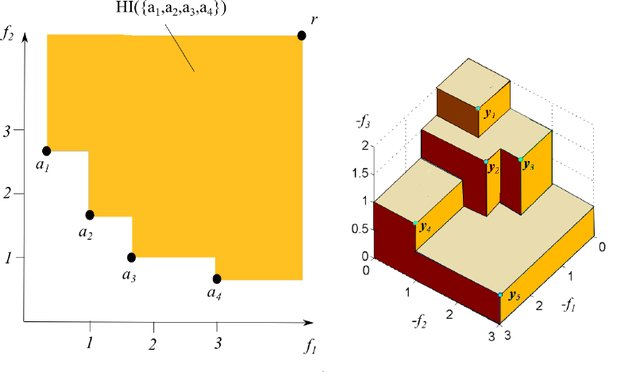
\includegraphics[width=0.55\textwidth]{HV.jpg}
%\caption{\scriptsize Mapeo del espacio de las variables (a) en el espacio objetivo (b)\footcite{alam2012diversity}.}
\end{figure}
\end{frame}

\begin{frame}{Distancia generacional}
\begin{itemize}
\justifying
\scriptsize
\item En el \citeyear{Joel:GD} \citeauthor{Joel:GD} propuso la distancia generacional (GD), el cual es un indicador unario del tipo Pareto \textit{non-compliant}.
\item \textcolor{red}{Requiere de un conjunto de referencia}, el cual es una discretización del frente de Pareto.
\item El GD calcula la distancia promedio de cada solución obtenido al punto de referencia más cercano.
\end{itemize}
\begin{equation*}
\scriptsize
\begin{split}
GD(A; R) = \frac{1}{|A|} \left (   \sum_{a \in A} d(a, R)^p \right)^{1/p}, \quad d(a, R) = \min_{r \in R} \sqrt{\sum_{i=1}^m (a_i - r_i)^2}
\end{split}
\end{equation*}
\begin{figure}[H]
\centering



\tikzset{every picture/.style={line width=0.75pt}} %set default line width to 0.75pt        

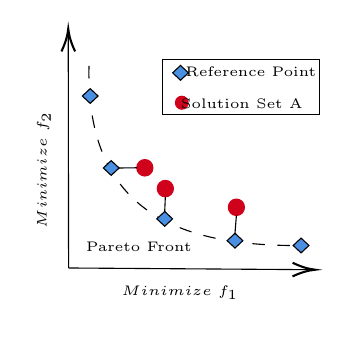
\begin{tikzpicture}[x=0.75pt,y=0.75pt,yscale=-1,xscale=1]
%uncomment if require: \path (0,235); %set diagram left start at 0, and has height of 235

%Straight Lines [id:da6645459220661805] 
\draw    (126.65,152.75) -- (126.49,39.47) ;
\draw [shift={(126.49,37.47)}, rotate = 449.92] [color={rgb, 255:red, 0; green, 0; blue, 0 }  ][line width=0.75]    (10.93,-3.29) .. controls (6.95,-1.4) and (3.31,-0.3) .. (0,0) .. controls (3.31,0.3) and (6.95,1.4) .. (10.93,3.29)   ;

%Straight Lines [id:da25810757520855776] 
\draw    (126.65,152.75) -- (243.5,153.57) ;
\draw [shift={(245.5,153.59)}, rotate = 180.4] [color={rgb, 255:red, 0; green, 0; blue, 0 }  ][line width=0.75]    (10.93,-3.29) .. controls (6.95,-1.4) and (3.31,-0.3) .. (0,0) .. controls (3.31,0.3) and (6.95,1.4) .. (10.93,3.29)   ;

%Curve Lines [id:da9217780493934806] 
\draw  [dash pattern={on 4.5pt off 4.5pt}]  (136.49,55.41) .. controls (134.85,129.62) and (185.36,142.75) .. (241.91,141.91) ;


%Shape: Ellipse [id:dp9288304297821606] 
\draw  [color={rgb, 255:red, 208; green, 2; blue, 27 }  ,draw opacity=1 ][fill={rgb, 255:red, 208; green, 2; blue, 27 }  ,fill opacity=1 ] (159.5,104.47) .. controls (159.5,102.29) and (161.24,100.51) .. (163.39,100.51) .. controls (165.54,100.51) and (167.29,102.29) .. (167.29,104.47) .. controls (167.29,106.66) and (165.54,108.44) .. (163.39,108.44) .. controls (161.24,108.44) and (159.5,106.66) .. (159.5,104.47) -- cycle ;
%Shape: Ellipse [id:dp3466831035198521] 
\draw  [color={rgb, 255:red, 208; green, 2; blue, 27 }  ,draw opacity=1 ][fill={rgb, 255:red, 208; green, 2; blue, 27 }  ,fill opacity=1 ] (203.61,123.51) .. controls (203.61,121.33) and (205.35,119.55) .. (207.5,119.55) .. controls (209.65,119.55) and (211.39,121.33) .. (211.39,123.51) .. controls (211.39,125.7) and (209.65,127.47) .. (207.5,127.47) .. controls (205.35,127.47) and (203.61,125.7) .. (203.61,123.51) -- cycle ;
%Shape: Ellipse [id:dp8431057514843725] 
\draw  [color={rgb, 255:red, 208; green, 2; blue, 27 }  ,draw opacity=1 ][fill={rgb, 255:red, 208; green, 2; blue, 27 }  ,fill opacity=1 ] (169.37,114.51) .. controls (169.37,112.32) and (171.11,110.54) .. (173.27,110.54) .. controls (175.42,110.54) and (177.16,112.32) .. (177.16,114.51) .. controls (177.16,116.69) and (175.42,118.47) .. (173.27,118.47) .. controls (171.11,118.47) and (169.37,116.69) .. (169.37,114.51) -- cycle ;
%Shape: Diamond [id:dp16787571758178776] 
\draw  [color={rgb, 255:red, 0; green, 0; blue, 0 }  ,draw opacity=1 ][fill={rgb, 255:red, 74; green, 144; blue, 226 }  ,fill opacity=1 ] (137.07,66.34) -- (140.86,69.89) -- (137.07,73.45) -- (133.28,69.89) -- cycle ;
%Shape: Diamond [id:dp8884066450256918] 
\draw  [color={rgb, 255:red, 0; green, 0; blue, 0 }  ,draw opacity=1 ][fill={rgb, 255:red, 74; green, 144; blue, 226 }  ,fill opacity=1 ] (147.19,101.02) -- (150.98,104.58) -- (147.19,108.13) -- (143.4,104.58) -- cycle ;
%Shape: Diamond [id:dp7101561956457161] 
\draw  [color={rgb, 255:red, 0; green, 0; blue, 0 }  ,draw opacity=1 ][fill={rgb, 255:red, 74; green, 144; blue, 226 }  ,fill opacity=1 ] (172.96,125.53) -- (176.75,129.09) -- (172.96,132.64) -- (169.17,129.09) -- cycle ;
%Shape: Diamond [id:dp3806535283252863] 
\draw  [color={rgb, 255:red, 0; green, 0; blue, 0 }  ,draw opacity=1 ][fill={rgb, 255:red, 74; green, 144; blue, 226 }  ,fill opacity=1 ] (206.83,136.04) -- (210.62,139.59) -- (206.83,143.15) -- (203.03,139.59) -- cycle ;
%Shape: Diamond [id:dp006261489471205639] 
\draw  [color={rgb, 255:red, 0; green, 0; blue, 0 }  ,draw opacity=1 ][fill={rgb, 255:red, 74; green, 144; blue, 226 }  ,fill opacity=1 ] (238.66,138.36) -- (242.46,141.91) -- (238.66,145.47) -- (234.87,141.91) -- cycle ;
%Straight Lines [id:da45493974031657336] 
\draw    (150.98,104.58) -- (159.5,104.47) ;


%Straight Lines [id:da5268787235096657] 
\draw    (172.96,125.53) -- (173.27,118.47) ;


%Straight Lines [id:da45090976417004924] 
\draw    (207.5,127.47) -- (206.83,136.04) ;


%Shape: Ellipse [id:dp4881097987438625] 
\draw  [color={rgb, 255:red, 208; green, 2; blue, 27 }  ,draw opacity=1 ][fill={rgb, 255:red, 208; green, 2; blue, 27 }  ,fill opacity=1 ] (178.13,73.14) .. controls (178.13,71.41) and (179.5,70.01) .. (181.2,70.01) .. controls (182.9,70.01) and (184.27,71.41) .. (184.27,73.14) .. controls (184.27,74.86) and (182.9,76.26) .. (181.2,76.26) .. controls (179.5,76.26) and (178.13,74.86) .. (178.13,73.14) -- cycle ;
%Shape: Rectangle [id:dp7606725757806145] 
\draw   (171.98,52.31) -- (247.5,52.31) -- (247.5,79) -- (171.98,79) -- cycle ;
%Shape: Diamond [id:dp5520874909126483] 
\draw  [color={rgb, 255:red, 0; green, 0; blue, 0 }  ,draw opacity=1 ][fill={rgb, 255:red, 74; green, 144; blue, 226 }  ,fill opacity=1 ] (180.58,55.18) -- (184.38,58.74) -- (180.58,62.29) -- (176.79,58.74) -- cycle ;

% Text Node
\draw (180.34,164.66) node  [font=\footnotesize]  {$Minimize\ f_{1}$};
% Text Node
\draw (114.77,105.46) node  [font=\footnotesize,rotate=-270.12]  {$Minimize\ f_{2}$};
% Text Node
\draw (160.49,142.48) node  [font=\tiny] [align=left] {Pareto Front};
% Text Node
\draw (210.22,73.49) node  [font=\small] [align=left] {{\tiny Solution Set A}};
% Text Node
\draw (214.5,58.31) node  [font=\small] [align=left] {{\tiny Reference Point}};


\end{tikzpicture}

%\includegraphics[width=0.45\textwidth]{Images/Fase_Remplazo_2.eps}
\caption{\scriptsize Ejemplo de la distancia generacional y un conjunto de referencia.} 
\end{figure}
\end{frame}


\begin{frame}{Desventajas de la distancia generacional}
\begin{itemize}
\justifying
\scriptsize
\item El conjunto aproximado puede no converger a todo el frente de Pareto y aún así se tendría una medición ``buena'' (ver figura \ref{fig:igd}).

\item Existe un sesgo al incrementar el número de puntos aproximados, es decir da valores menores del GD al aumentar la cantidad de soluciones pero sin mejorar la calidad de las aproximaciones\footcite{Joel:HausdorffDistance}.
%\begin{equation*}
%\begin{split}
%& GD(a, R) = \frac{1}{|A|} \left (   \sum_{a \in A} d(a, R)^p \right)^{1/p} = \frac{||(1,...,1)^T ||_p}{|A|} = \frac{(|A|)^{1/p}}{|A|} \\
%& lim_{|A| \rightarrow \inf} GD(a, R) = 0 \\
%\end{split}
%\end{equation*}
\item ¿Cómo se puede mejorar?
\end{itemize}
\begin{figure}[H]
\centering



\tikzset{every picture/.style={line width=0.75pt}} %set default line width to 0.75pt        

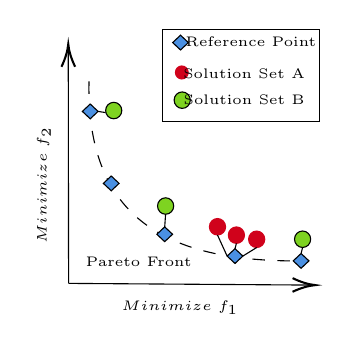
\begin{tikzpicture}[x=0.75pt,y=0.75pt,yscale=-1,xscale=1]
%uncomment if require: \path (0,235); %set diagram left start at 0, and has height of 235

%Straight Lines [id:da8717354133525324] 
\draw    (420.65,153.75) -- (420.49,40.47) ;
\draw [shift={(420.49,38.47)}, rotate = 449.92] [color={rgb, 255:red, 0; green, 0; blue, 0 }  ][line width=0.75]    (10.93,-3.29) .. controls (6.95,-1.4) and (3.31,-0.3) .. (0,0) .. controls (3.31,0.3) and (6.95,1.4) .. (10.93,3.29)   ;

%Straight Lines [id:da6788473220220854] 
\draw    (420.65,153.75) -- (537.5,154.57) ;
\draw [shift={(539.5,154.59)}, rotate = 180.4] [color={rgb, 255:red, 0; green, 0; blue, 0 }  ][line width=0.75]    (10.93,-3.29) .. controls (6.95,-1.4) and (3.31,-0.3) .. (0,0) .. controls (3.31,0.3) and (6.95,1.4) .. (10.93,3.29)   ;

%Curve Lines [id:da2578618754086526] 
\draw  [dash pattern={on 4.5pt off 4.5pt}]  (430.49,56.41) .. controls (428.85,130.62) and (479.36,143.75) .. (535.91,142.91) ;


%Shape: Ellipse [id:dp791999357308242] 
\draw  [color={rgb, 255:red, 208; green, 2; blue, 27 }  ,draw opacity=1 ][fill={rgb, 255:red, 208; green, 2; blue, 27 }  ,fill opacity=1 ] (488.5,126.47) .. controls (488.5,124.29) and (490.24,122.51) .. (492.39,122.51) .. controls (494.54,122.51) and (496.29,124.29) .. (496.29,126.47) .. controls (496.29,128.66) and (494.54,130.44) .. (492.39,130.44) .. controls (490.24,130.44) and (488.5,128.66) .. (488.5,126.47) -- cycle ;
%Shape: Ellipse [id:dp9676691887328452] 
\draw  [color={rgb, 255:red, 208; green, 2; blue, 27 }  ,draw opacity=1 ][fill={rgb, 255:red, 208; green, 2; blue, 27 }  ,fill opacity=1 ] (497.61,130.51) .. controls (497.61,128.33) and (499.35,126.55) .. (501.5,126.55) .. controls (503.65,126.55) and (505.39,128.33) .. (505.39,130.51) .. controls (505.39,132.7) and (503.65,134.47) .. (501.5,134.47) .. controls (499.35,134.47) and (497.61,132.7) .. (497.61,130.51) -- cycle ;
%Shape: Ellipse [id:dp5116089282119083] 
\draw  [color={rgb, 255:red, 208; green, 2; blue, 27 }  ,draw opacity=1 ][fill={rgb, 255:red, 208; green, 2; blue, 27 }  ,fill opacity=1 ] (507.37,132.51) .. controls (507.37,130.32) and (509.11,128.54) .. (511.27,128.54) .. controls (513.42,128.54) and (515.16,130.32) .. (515.16,132.51) .. controls (515.16,134.69) and (513.42,136.47) .. (511.27,136.47) .. controls (509.11,136.47) and (507.37,134.69) .. (507.37,132.51) -- cycle ;
%Shape: Diamond [id:dp9404744531551759] 
\draw  [color={rgb, 255:red, 0; green, 0; blue, 0 }  ,draw opacity=1 ][fill={rgb, 255:red, 74; green, 144; blue, 226 }  ,fill opacity=1 ] (431.07,67.34) -- (434.86,70.89) -- (431.07,74.45) -- (427.28,70.89) -- cycle ;
%Shape: Diamond [id:dp1840229468184298] 
\draw  [color={rgb, 255:red, 0; green, 0; blue, 0 }  ,draw opacity=1 ][fill={rgb, 255:red, 74; green, 144; blue, 226 }  ,fill opacity=1 ] (441.19,102.02) -- (444.98,105.58) -- (441.19,109.13) -- (437.4,105.58) -- cycle ;
%Shape: Diamond [id:dp7181430347383788] 
\draw  [color={rgb, 255:red, 0; green, 0; blue, 0 }  ,draw opacity=1 ][fill={rgb, 255:red, 74; green, 144; blue, 226 }  ,fill opacity=1 ] (466.96,126.53) -- (470.75,130.09) -- (466.96,133.64) -- (463.17,130.09) -- cycle ;
%Shape: Diamond [id:dp0076213596461021105] 
\draw  [color={rgb, 255:red, 0; green, 0; blue, 0 }  ,draw opacity=1 ][fill={rgb, 255:red, 74; green, 144; blue, 226 }  ,fill opacity=1 ] (500.83,137.04) -- (504.62,140.59) -- (500.83,144.15) -- (497.03,140.59) -- cycle ;
%Shape: Diamond [id:dp3966825993991798] 
\draw  [color={rgb, 255:red, 0; green, 0; blue, 0 }  ,draw opacity=1 ][fill={rgb, 255:red, 74; green, 144; blue, 226 }  ,fill opacity=1 ] (532.66,139.36) -- (536.46,142.91) -- (532.66,146.47) -- (528.87,142.91) -- cycle ;
%Shape: Ellipse [id:dp8366972743499659] 
\draw  [color={rgb, 255:red, 208; green, 2; blue, 27 }  ,draw opacity=1 ][fill={rgb, 255:red, 208; green, 2; blue, 27 }  ,fill opacity=1 ] (472.13,52.14) .. controls (472.13,50.41) and (473.5,49.01) .. (475.2,49.01) .. controls (476.9,49.01) and (478.27,50.41) .. (478.27,52.14) .. controls (478.27,53.86) and (476.9,55.26) .. (475.2,55.26) .. controls (473.5,55.26) and (472.13,53.86) .. (472.13,52.14) -- cycle ;
%Shape: Rectangle [id:dp9875854969558264] 
\draw   (465.98,31.31) -- (541.5,31.31) -- (541.5,75.72) -- (465.98,75.72) -- cycle ;
%Shape: Diamond [id:dp12687480943241192] 
\draw  [color={rgb, 255:red, 0; green, 0; blue, 0 }  ,draw opacity=1 ][fill={rgb, 255:red, 74; green, 144; blue, 226 }  ,fill opacity=1 ] (474.58,34.18) -- (478.38,37.74) -- (474.58,41.29) -- (470.79,37.74) -- cycle ;
%Shape: Ellipse [id:dp7460760771460382] 
\draw  [color={rgb, 255:red, 0; green, 0; blue, 0 }  ,draw opacity=1 ][fill={rgb, 255:red, 126; green, 211; blue, 33 }  ,fill opacity=1 ] (529.5,132.47) .. controls (529.5,130.29) and (531.24,128.51) .. (533.39,128.51) .. controls (535.54,128.51) and (537.29,130.29) .. (537.29,132.47) .. controls (537.29,134.66) and (535.54,136.44) .. (533.39,136.44) .. controls (531.24,136.44) and (529.5,134.66) .. (529.5,132.47) -- cycle ;
%Shape: Ellipse [id:dp8222601223763368] 
\draw  [color={rgb, 255:red, 0; green, 0; blue, 0 }  ,draw opacity=1 ][fill={rgb, 255:red, 126; green, 211; blue, 33 }  ,fill opacity=1 ] (438.5,70.47) .. controls (438.5,68.29) and (440.24,66.51) .. (442.39,66.51) .. controls (444.54,66.51) and (446.29,68.29) .. (446.29,70.47) .. controls (446.29,72.66) and (444.54,74.44) .. (442.39,74.44) .. controls (440.24,74.44) and (438.5,72.66) .. (438.5,70.47) -- cycle ;
%Shape: Ellipse [id:dp5535523746552888] 
\draw  [color={rgb, 255:red, 0; green, 0; blue, 0 }  ,draw opacity=1 ][fill={rgb, 255:red, 126; green, 211; blue, 33 }  ,fill opacity=1 ] (463.5,116.47) .. controls (463.5,114.29) and (465.24,112.51) .. (467.39,112.51) .. controls (469.54,112.51) and (471.29,114.29) .. (471.29,116.47) .. controls (471.29,118.66) and (469.54,120.44) .. (467.39,120.44) .. controls (465.24,120.44) and (463.5,118.66) .. (463.5,116.47) -- cycle ;
%Straight Lines [id:da3248368940477697] 
\draw    (434.86,70.89) -- (438.5,71.47) ;


%Straight Lines [id:da5912697186863101] 
\draw    (467.39,120.44) -- (466.96,126.53) ;


%Straight Lines [id:da6656789090734234] 
\draw    (533.39,136.44) -- (532.66,139.36) ;


%Straight Lines [id:da4766593569740376] 
\draw    (492.39,130.44) -- (497.03,140.59) ;


%Straight Lines [id:da5765204277329508] 
\draw    (501.5,134.47) -- (500.83,137.04) ;


%Straight Lines [id:da5373571677163032] 
\draw    (511.27,136.47) -- (504.62,140.59) ;


%Shape: Ellipse [id:dp9862032948376587] 
\draw  [color={rgb, 255:red, 0; green, 0; blue, 0 }  ,draw opacity=1 ][fill={rgb, 255:red, 126; green, 211; blue, 33 }  ,fill opacity=1 ] (471.5,65.47) .. controls (471.5,63.29) and (473.24,61.51) .. (475.39,61.51) .. controls (477.54,61.51) and (479.29,63.29) .. (479.29,65.47) .. controls (479.29,67.66) and (477.54,69.44) .. (475.39,69.44) .. controls (473.24,69.44) and (471.5,67.66) .. (471.5,65.47) -- cycle ;

% Text Node
\draw (474.34,165.66) node  [font=\footnotesize]  {$Minimize\ f_{1}$};
% Text Node
\draw (408.77,106.46) node  [font=\footnotesize,rotate=-270.12]  {$Minimize\ f_{2}$};
% Text Node
\draw (454.49,143.48) node  [font=\tiny] [align=left] {Pareto Front};
% Text Node
\draw (505.22,52.49) node  [font=\small] [align=left] {{\tiny Solution Set A}};
% Text Node
\draw (508.5,37.31) node  [font=\small] [align=left] {{\tiny Reference Point}};
% Text Node
\draw (505.22,65.49) node  [font=\small] [align=left] {{\tiny Solution Set B}};


\end{tikzpicture}

%\includegraphics[width=0.45\textwidth]{Images/Fase_Remplazo_2.eps}
\caption{\scriptsize Ejemplo de una desventaja de la distancia generacional.} \label{fig:igd}
\end{figure}


\end{frame}


\begin{frame}{Distancia generacional invertida}
\begin{itemize}
\justifying
\scriptsize
\item A diferencia del GD, la Distancia Generacional Invertida (IGD) es la distancia promedio de cada punto de referencia a su solución más cercana del conjunto aproximado.
%\item La métrica sigue siendo Pareto \textit{non-compliant}.
\end{itemize}
\begin{equation*}
\scriptsize
\begin{split}
IGD(A; R) = \frac{1}{|R|} \left (   \sum_{r \in R} d(r, A)^p \right)^{1/p}, \quad d(r, A) = \min_{a \in A} \sqrt{\sum_{i=1}^m (r_i - a_i)^2}
\end{split}
\end{equation*}

\begin{figure}[H]
\centering
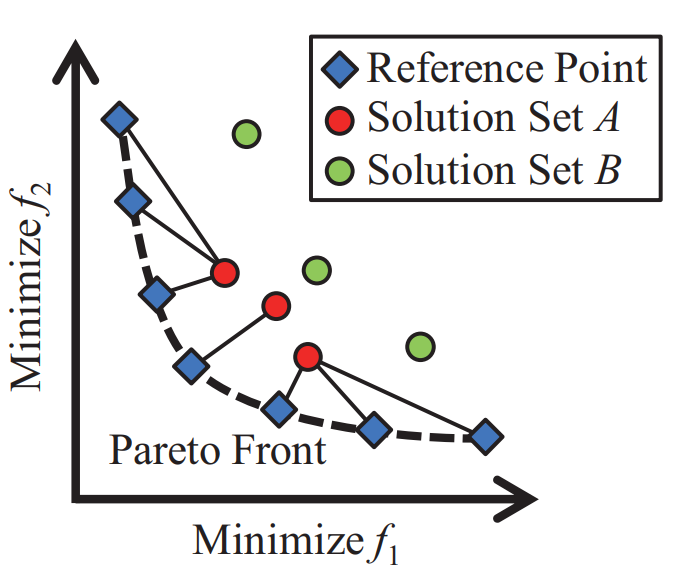
\includegraphics[width=0.4\textwidth]{igd_1.png}
\caption{\scriptsize Ejemplo de la distancia generacional invertida.\footcite{ishibuchi2016sensitivity}.}
\end{figure}
\end{frame}


\begin{frame}{Desventajas de la distancia generacional invertida}
\begin{itemize}
\justifying
\scriptsize
\item La métrica sigue siendo Pareto \textit{non-compliant}, por lo tanto existen situaciones en que un conjunto de soluciones alejado del frente pueda generar mejores valores que un conjunto más cercano del frente.
\item Se puede observar en la figura \ref{fig:igd_fail} que a pesar de que la solución $\boldsymbol{b}$ es dominada por la solución $\boldsymbol{a}$, la distancia de un punto de referencia $\boldsymbol{z}$ a $\boldsymbol{b}$ puede ser menor que la distancia de $\boldsymbol{z}$ a $\boldsymbol{a}$.
\item ¿Cómo se puede mejorar?
\end{itemize}
\begin{figure}[H]
\centering
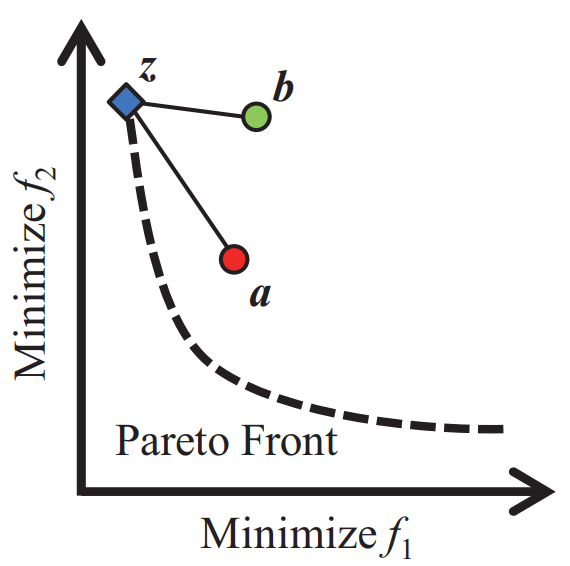
\includegraphics[width=0.3\textwidth]{igd_2.png}
\caption{\scriptsize Desventaja de la métrica IGD.\footcite{ishibuchi2016sensitivity}.} \label{fig:igd_fail}
\end{figure}
\end{frame}



\begin{frame}{Distancias generacional invertida modificada}
\begin{itemize}
\justifying
\scriptsize
\item Propuesta por \citeauthor{Joel:IGDPlus_And_GDPlus} en el \citeyear{Joel:IGDPlus_And_GDPlus}, es considerada como débilmente \textit{Pareto Compliant}.
\item Si una solución es dominada por un punto de referencia se utiliza la distancia euclideana.
\item Si la solución y el punto de referencia son no dominados entre sí, entonce se calcula la distancia mínima desde el punto de referencia a la región no dominada.
\end{itemize}
\begin{equation*}
\scriptsize
\begin{split}
IGD^+(A; R) = \frac{1}{|R|} \left (   \sum_{r \in R} d^+(r, A)^p \right)^{1/p}, \quad d^+ = \min_{a \in A} \sqrt{\sum_{i=1}^m (max\{ a_i - z_i, 0\})^2}
\end{split}
\end{equation*}


\begin{figure}[H]
\centering
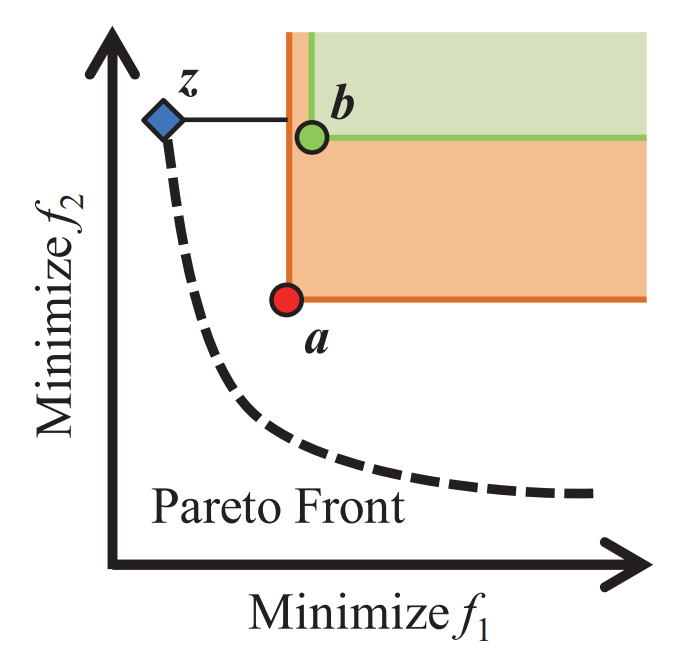
\includegraphics[width=0.25\textwidth]{igd_3.png}
\caption{\scriptsize Distancia generacional invertida modificada ($IGD^+$).\footcite{ishibuchi2016sensitivity}.}
\end{figure}
\end{frame}

\begin{frame}{Distancias}

% Please add the following required packages to your document preamble:
% \usepackage{graphicx}
\begin{table}[]
\resizebox{\textwidth}{!}{%
\begin{tabular}{c|c}
$IGD(A; R) =  \frac{1}{|R|} \left (  \sum_{r \in R} d(r, A)^p \right)^{1/p}$ & $IGD^+(A; R)= \frac{1}{|R|}\left (   \sum_{r \in R} d^+(r, A)^p \right)^{1/p}$ \\ \\
$d = \min_{a \in A} \sqrt{\sum_{i=1}^m (a_i - r_i)^2}$ & $d^+ = \min_{a \in A} \sqrt{\sum_{i=1}^m (max\{ a_i - z_i, 0\})^2}$
\end{tabular}%
}
\end{table}
\begin{figure}[H]
\centering
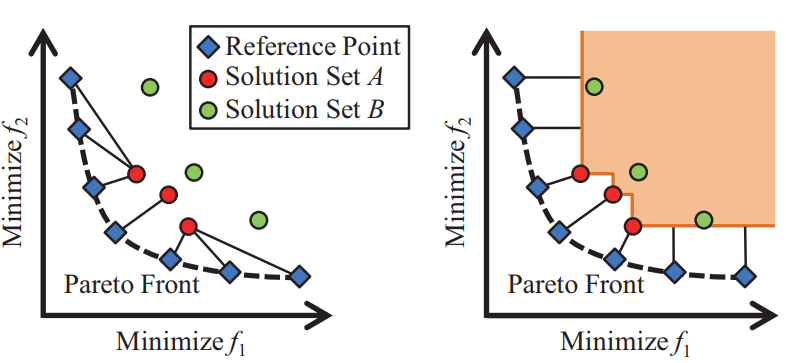
\includegraphics[width=0.7\textwidth]{igd.png}
\caption{\scriptsize Ejemplo de las métricas $IGD$ (izquierda) e $IGD^+$ (derecha).\footcite{ishibuchi2016sensitivity}.}
\end{figure}
\end{frame}



\section{Problemas de prueba en multi-objetivo}
\begin{frame}{Problemas de prueba en el ámbito multi-objetivo}
\begin{itemize}
   \item ZDT, \citeauthor{Joel:ZDT}, \citeyear{Joel:ZDT}.%, únicamente de dos objetivos, escalables en las variables.
   \item DTLZ, \citeauthor{Joel:DTLZ_1}, (versión 1 \citeyear{Joel:DTLZ_1}, versión 2 \citeyear{Joel:DTLZ_2}).%, escalables en los objetivos y las variables.
   \item WFG, \citeauthor{Joel:WFG_Main}, \citeyear{Joel:WFG_Main}.%, escalables en los objetivos y las variables.
   \item UF, \citeauthor{Joel:CEC2009}, \citeyear{Joel:CEC2009}.%, únicamente de dos objetivos (UF1-UF7) y tres objetivos (UF8-UF10), escalables en las variables.
\end{itemize}
\end{frame}


\begin{frame}{Problemas de prueba DTLZ}
\begin{itemize}
   \scriptsize
   \item Estos problemas son escalables en los objetivos y las variables.
   \item Existen dos versiones diseñadas por los mismos autores, en el \citeyear{Joel:DTLZ_1} y en el \citeyear{Joel:DTLZ_2}.
   \item Los óptimos globales están ubicados en el centro del espacio de búsqueda o en los límites.
   \item Para todos los problemas, el óptimo global tiene los mismos valores de parámetros para distintas variables.
\end{itemize}
\begin{figure}[H]
\begin{tabular}{c c}
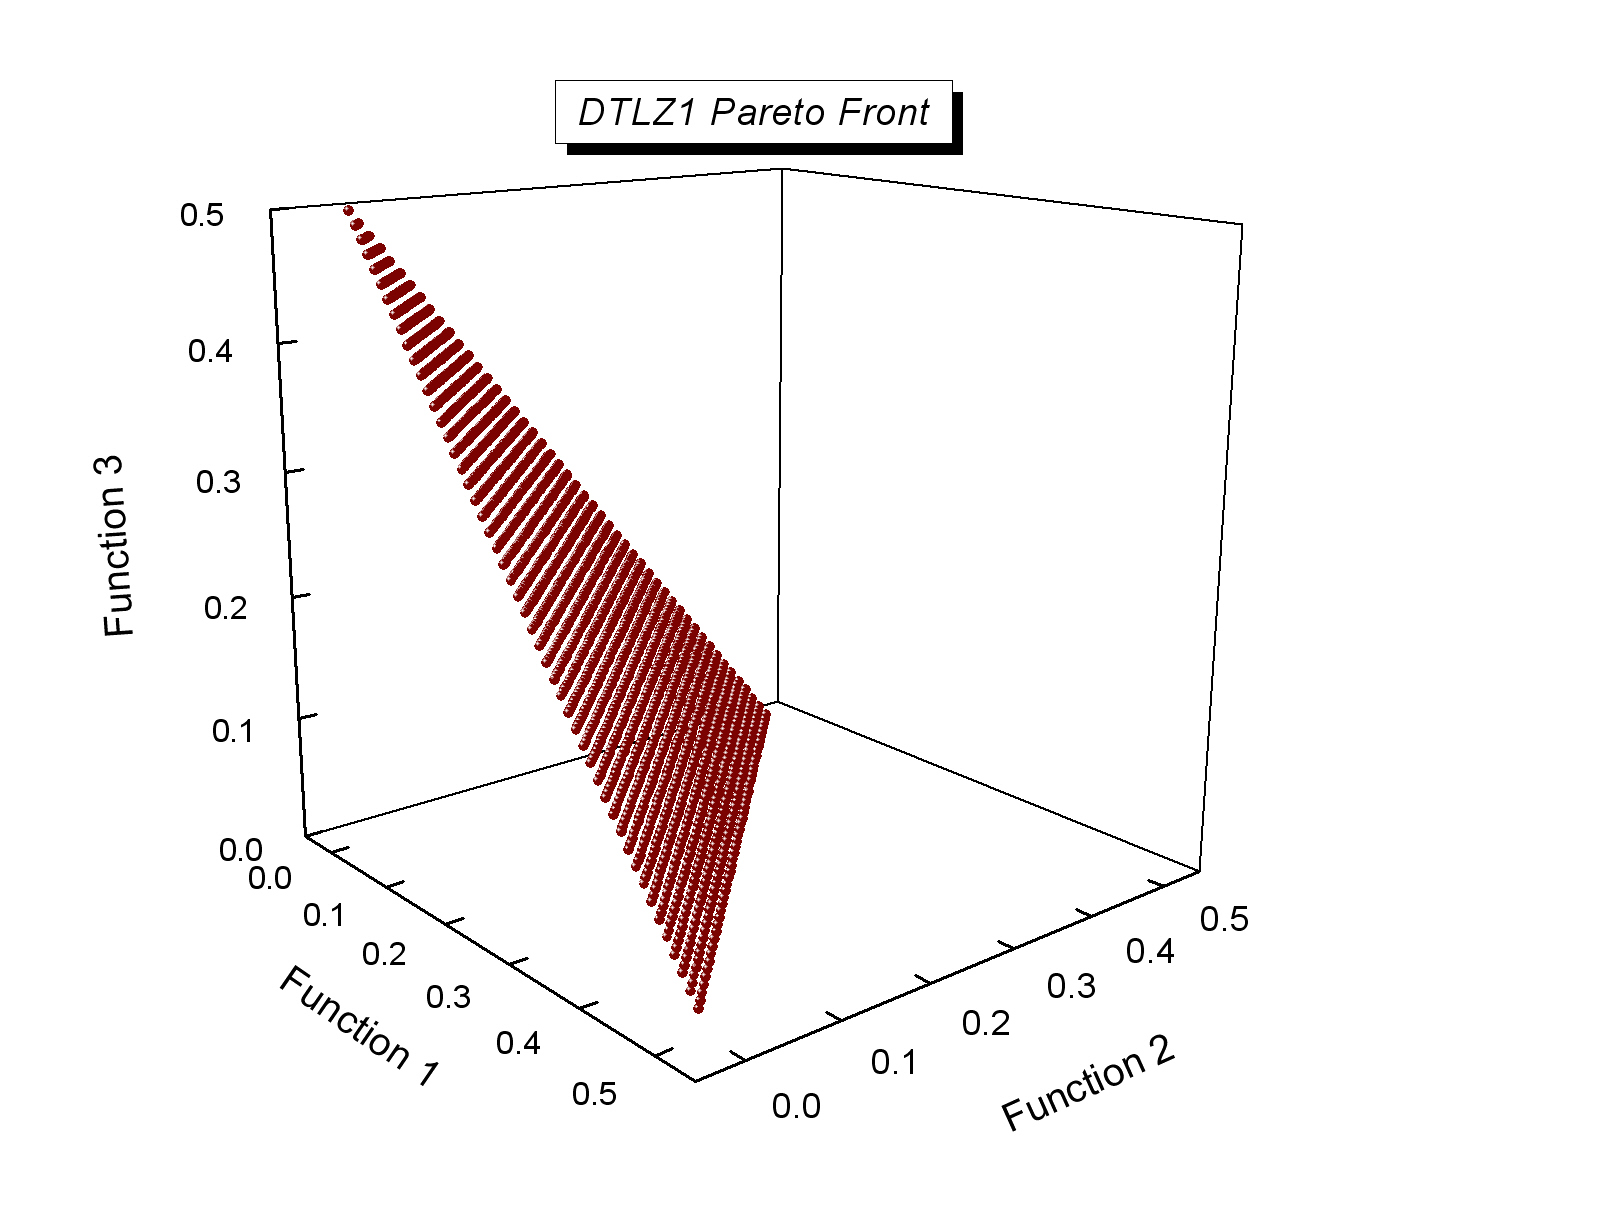
\includegraphics[width=0.3\textwidth]{DTLZ1.jpg}     &  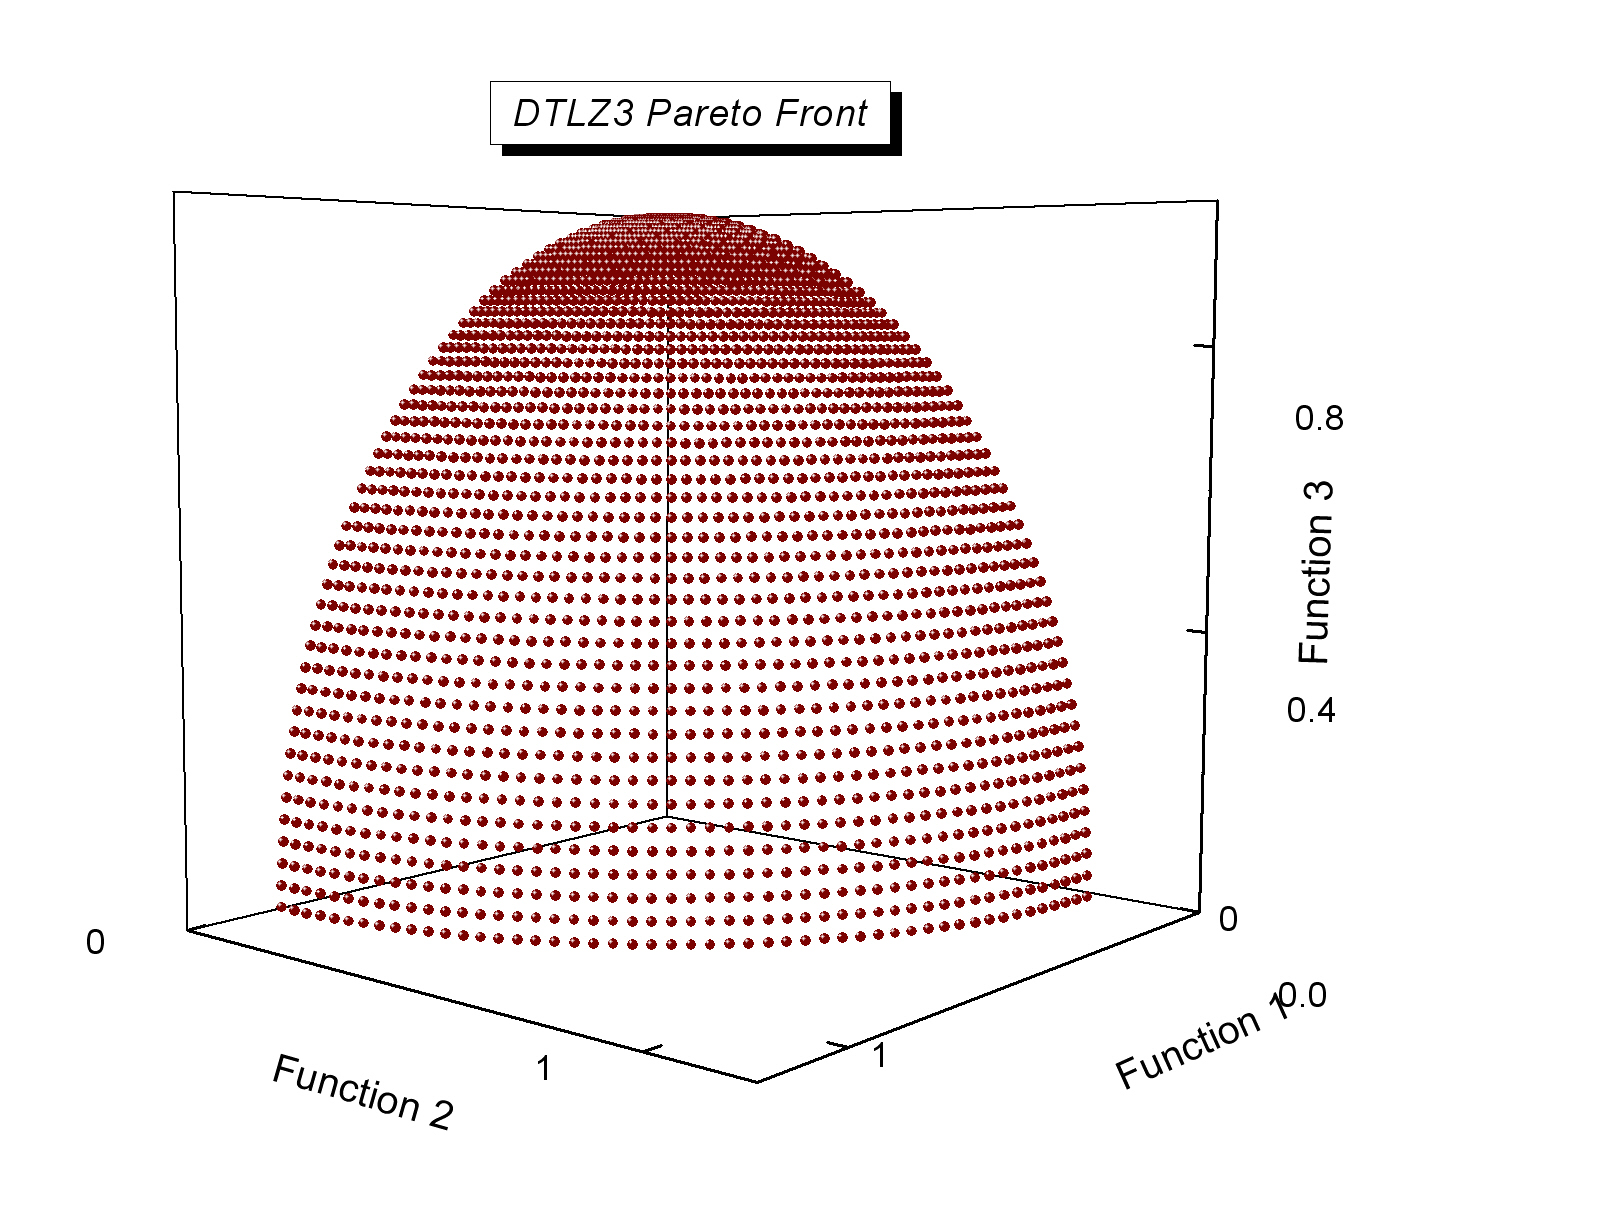
\includegraphics[width=0.3\textwidth]{DTLZ3.jpg} \\
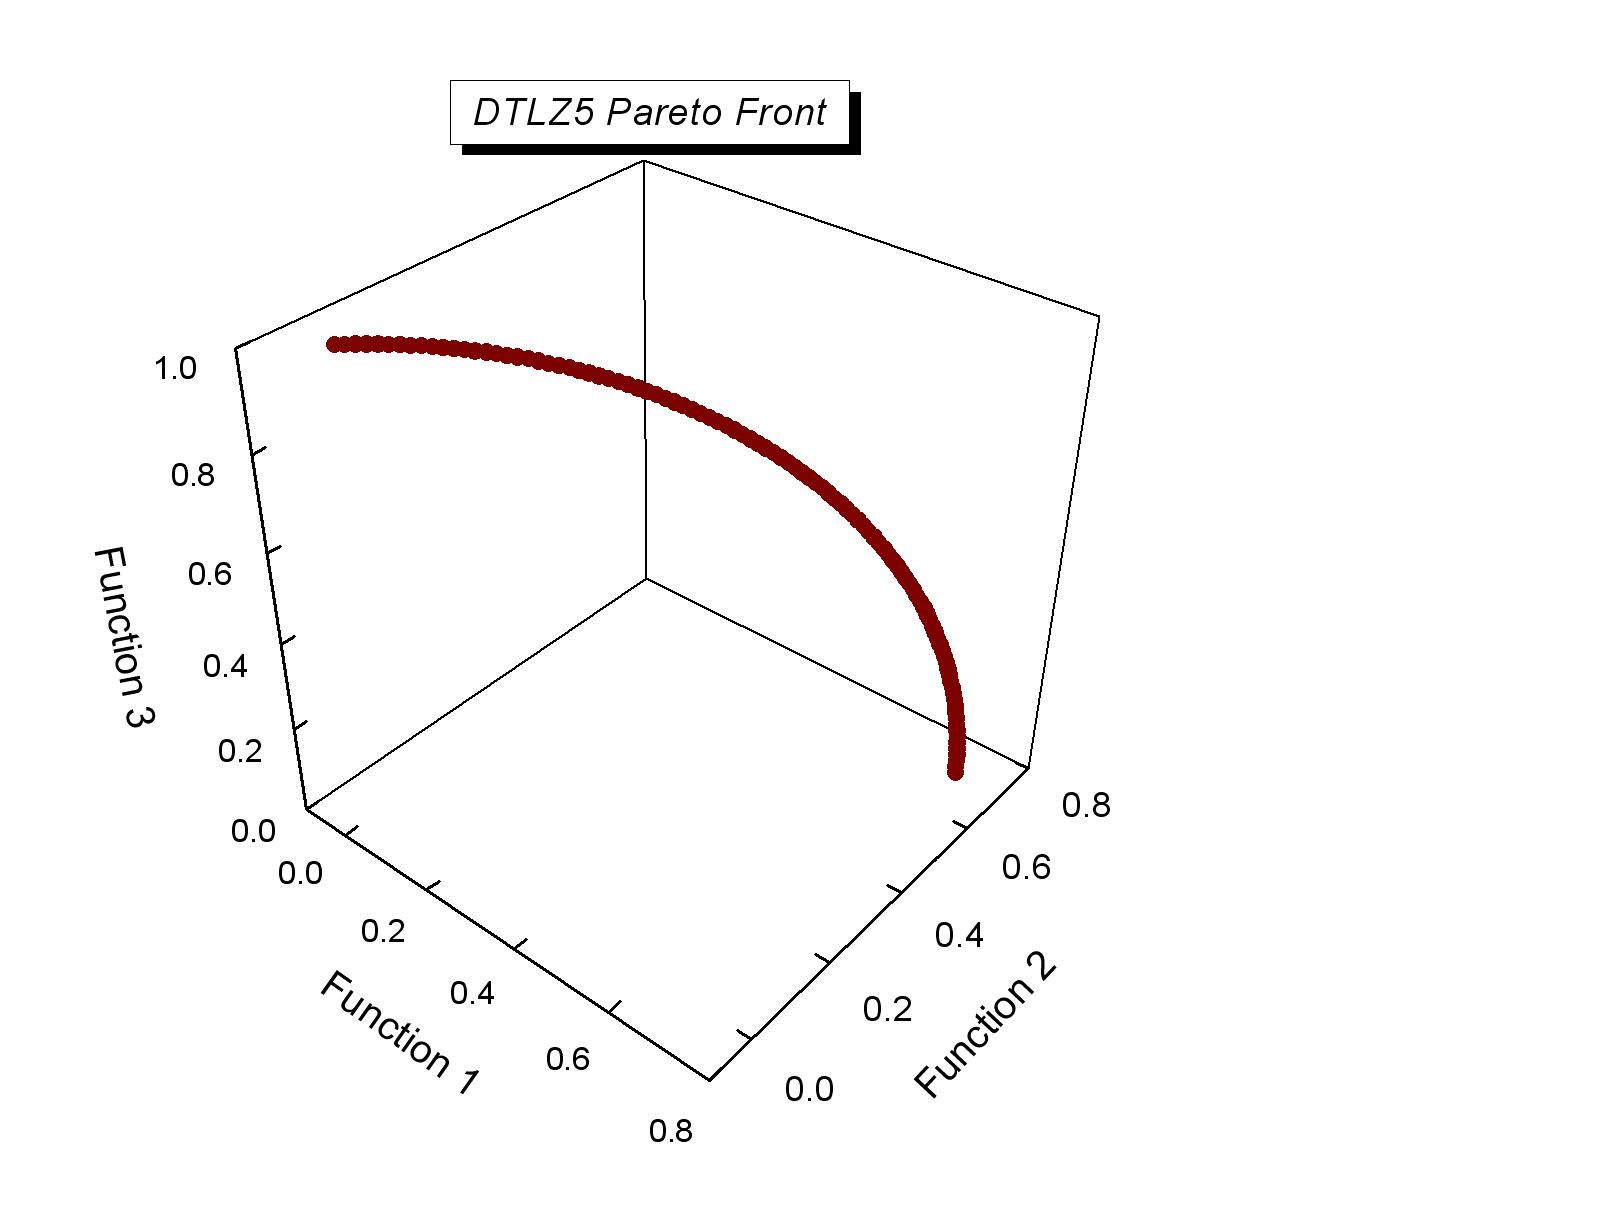
\includegraphics[width=0.3\textwidth]{DTLZ5.jpg}     &  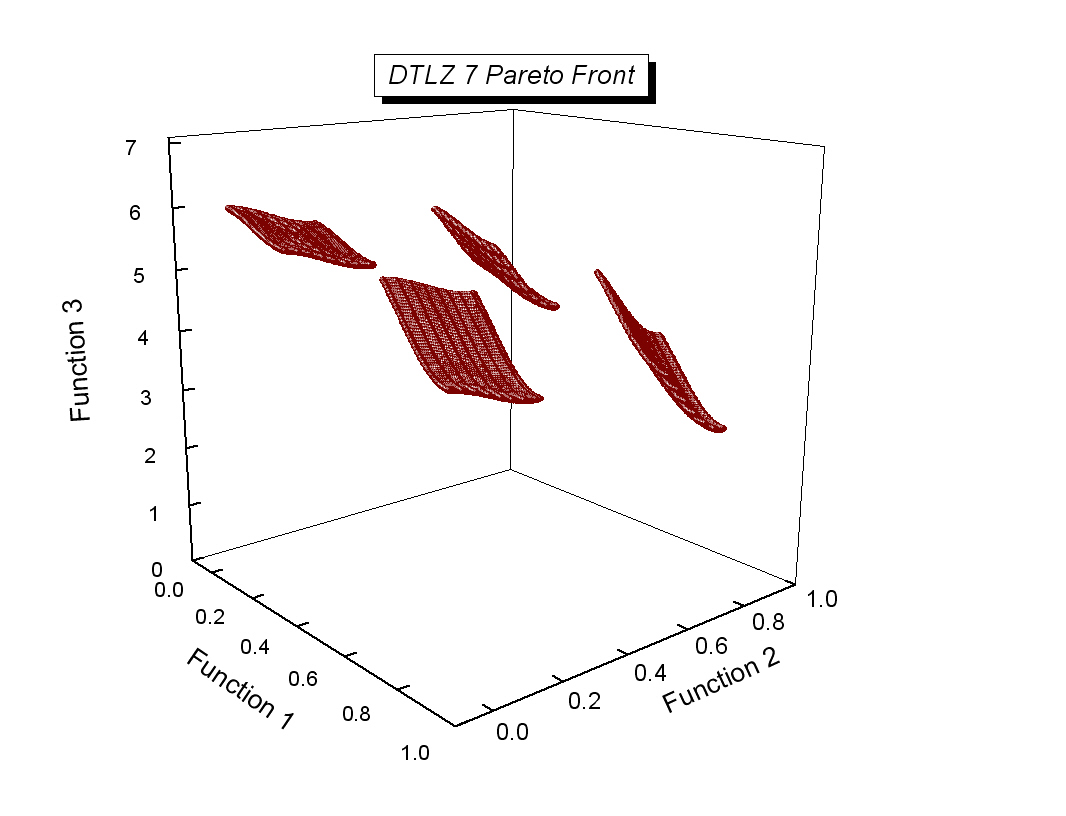
\includegraphics[width=0.3\textwidth]{DTLZ7.jpg} \\
\end{tabular}
\centering
\caption{\scriptsize Frente de Pareto discretizado.}
\end{figure}

\end{frame}


\begin{frame}{Problemas de prueba \textit{Walking Fish Group} WFG}
\begin{itemize}
\scriptsize
   \item Estos problemas son escalables en los objetivos y las variables.
   \item El generador de problemas de prueba WFG fue propuesto por \citeauthor{Joel:WFG} en el \citeyear{Joel:WFG}.
   \item A pesar de que es un generador de problemas, popularmente se utilizan nueve problemas de prueba.
   \item Los problemas WFG dividen el espaco de las variables de decisión en dos subconjuntos: los parámetros de distancia y los parámetros de posición.
\end{itemize}
\begin{figure}[H]
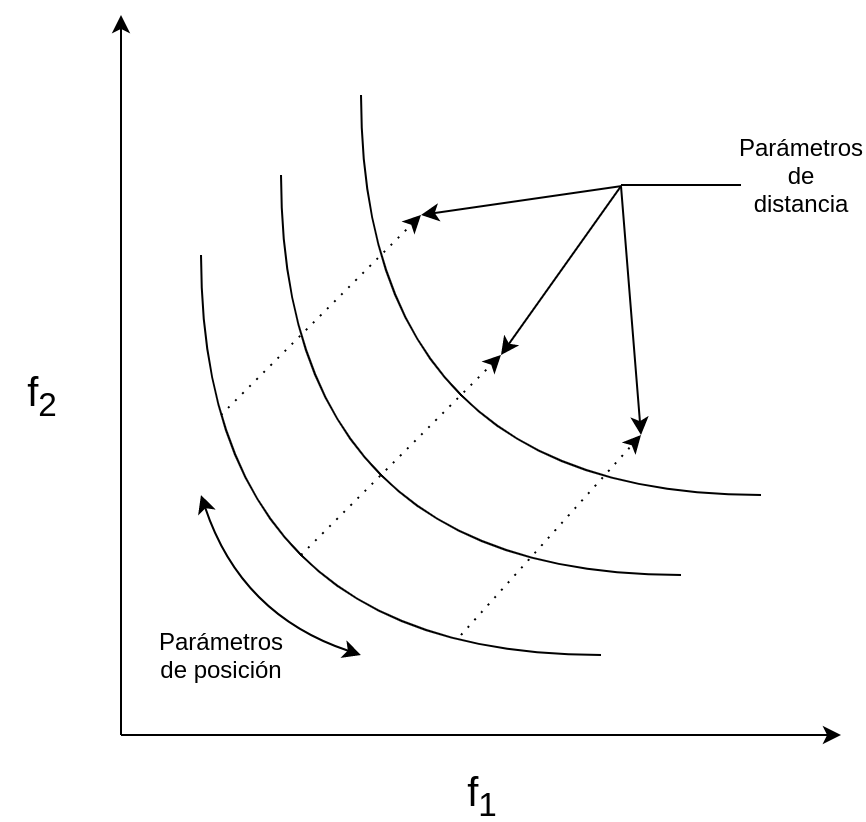
\includegraphics[width=0.45\textwidth]{pos_dist.png}
\centering
\caption{\scriptsize Parámetros de posición y distancia WFG.}
\end{figure}
\end{frame}


\begin{frame}{Unconstrained Functions UF}
\begin{itemize}
\scriptsize
   \item Estos son únicamente de dos objetivos (UF1-UF7) y tres objetivos (UF8-UF10), además son escalables en las variables.
   \item Este conjunto de prueba fue propuesto en el Congreso de Cómputo Evolutivo (CEC 2009) por \citeauthor{Joel:CEC2009}.
   \item Este tipo de problemas aún se consideran un reto para los optimizadores multi-objetivo más recientes.
\end{itemize}
\begin{figure}[H]
\begin{tabular}{c c}
\includegraphics[width=0.4\textwidth]{UF1.eps}     &  \includegraphics[width=0.4\textwidth]{UF6.eps} \\
\includegraphics[width=0.4\textwidth]{UF9.eps}     &  \includegraphics[width=0.4\textwidth]{UF10.eps} \\
\end{tabular}
\centering
\caption{\scriptsize Frente de Pareto y conjunto de Pareto.}
\end{figure}

\end{frame}



\begin{frame}{Superficie de alcance}
\begin{itemize}
\item Una superficie de alcance o superficie de cubrimiento es una descripción de la distribución alcanzada en base a un conjunto de soluciones.
\item Es un gráfico que muestra un resumen de una cantidad de soluciones en varias medidas descriptivas y considerando la relación de dominancia.
\end{itemize}
\begin{figure}[H]
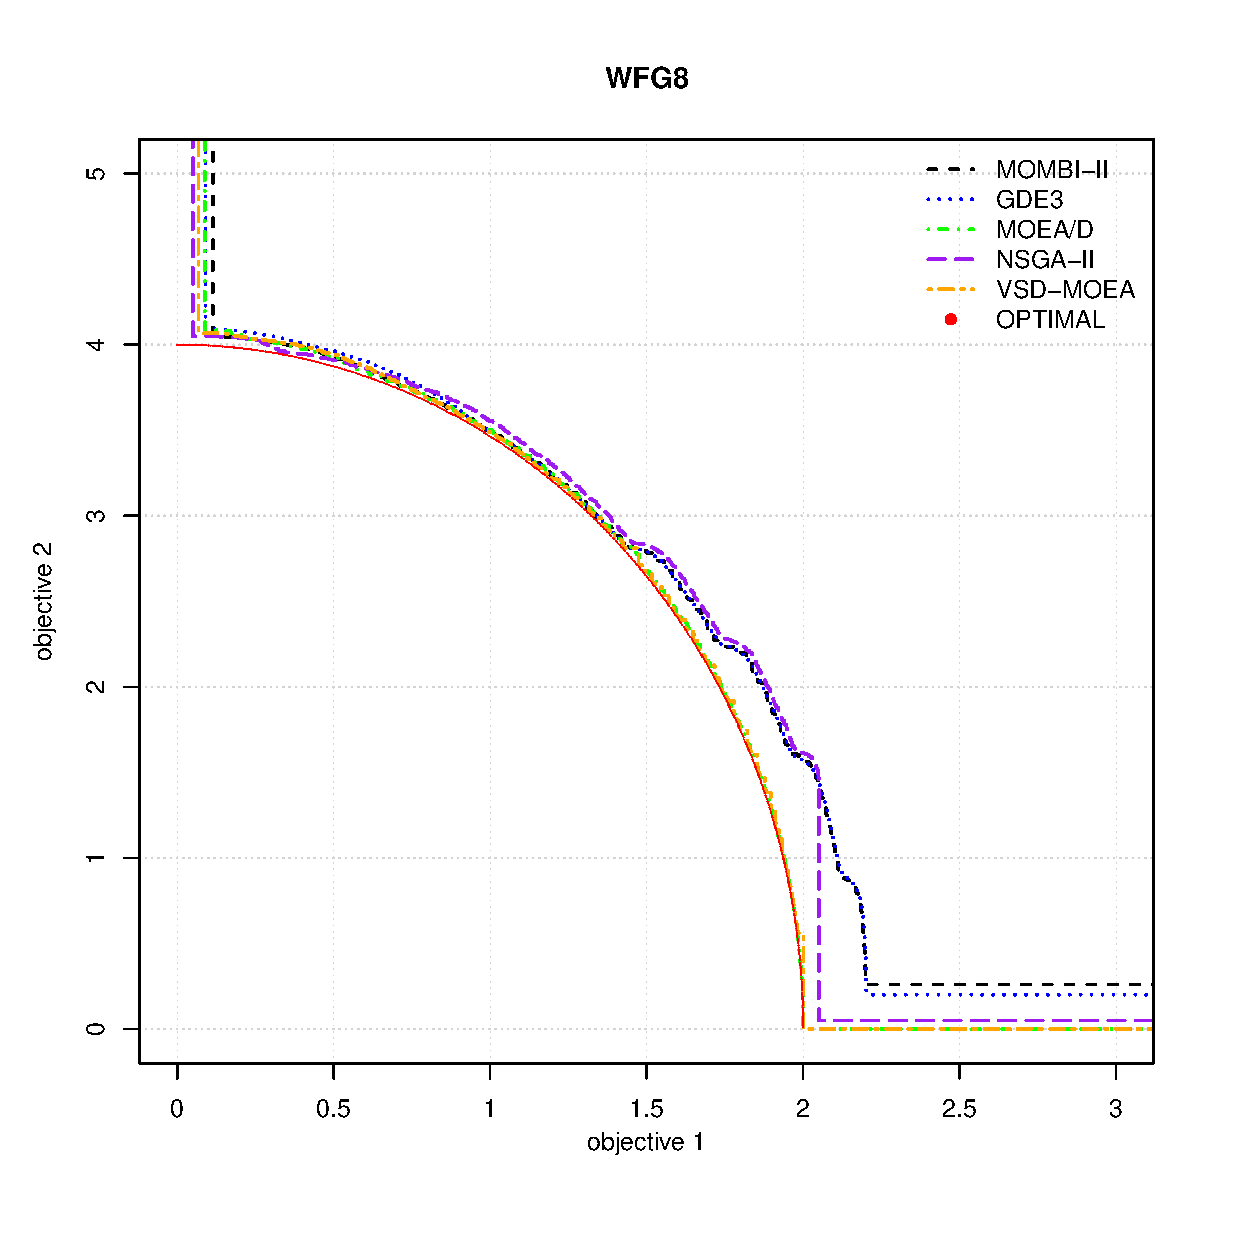
\includegraphics[width=0.4\textwidth]{superficie_alcance_WFG8.eps}
\centering
\caption{\scriptsize Superficie de alcance al $50\%$ de cinco algoritmos del estado-del-arte considerando el resultado de 35 ejecuciones y el problema WFG8.}
\end{figure}
\end{frame}


\begin{frame}{Diferencia de la superficie de alcance}
\begin{itemize}
\item Proporciona una diferencia estadística entre los resultados generados por dos algoritmos.
\end{itemize}
\begin{figure}[H]
 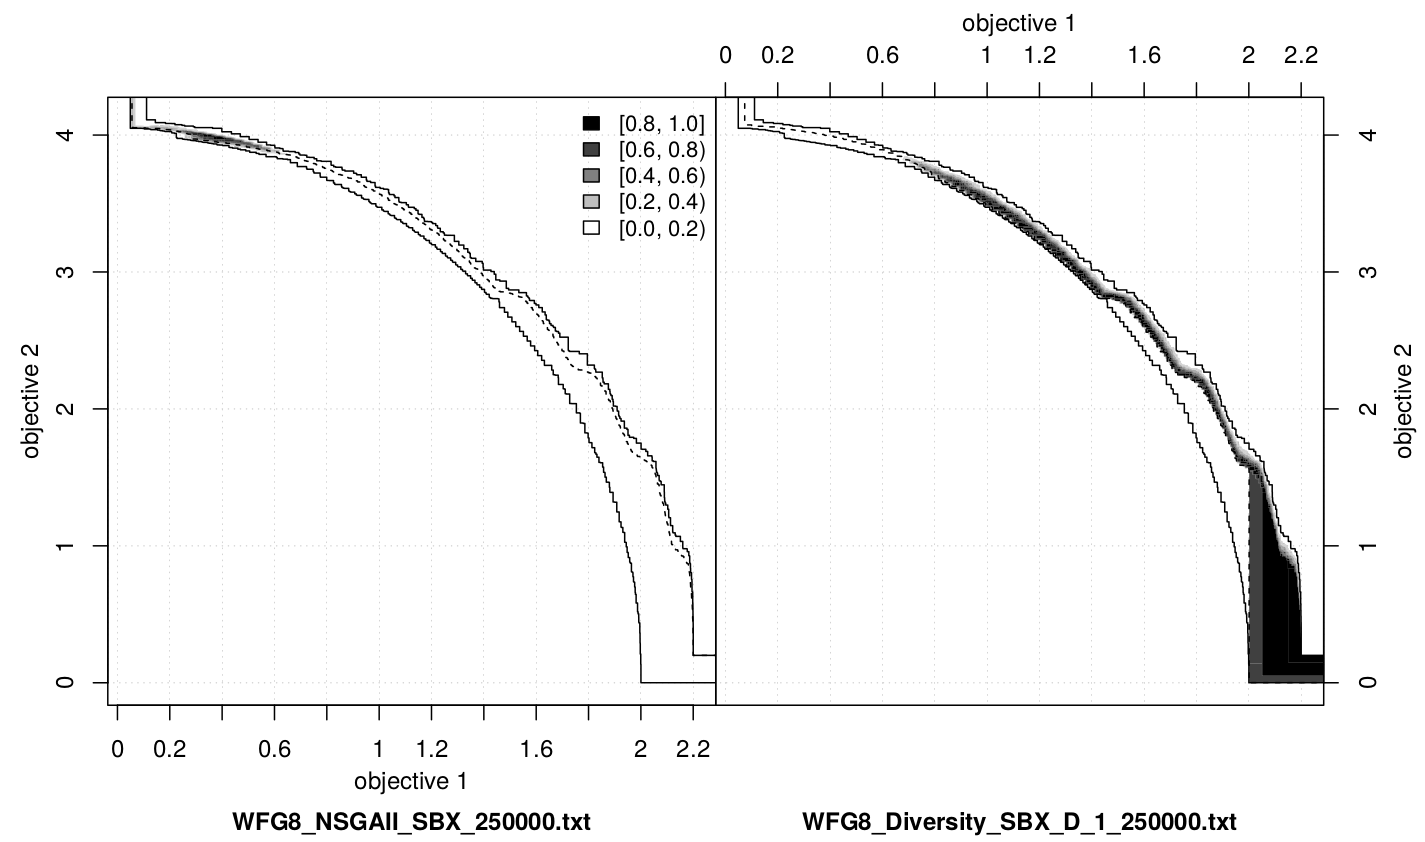
\includegraphics[width=0.8\textwidth]{diff_plot.png} 
\centering
\caption{\scriptsize Diferencia estadística de dos algoritmos considerando 35 ejecuciones y el problema WFG8.}
\end{figure}

\end{frame}



\begin{frame}{Pruebas estadísticas}
\begin{itemize}
\item Las pruebas estadísticas se realizan comparando resultados de los algoritmos por pares.
\end{itemize}
\begin{figure}[H]
\begin{tabular}{c}
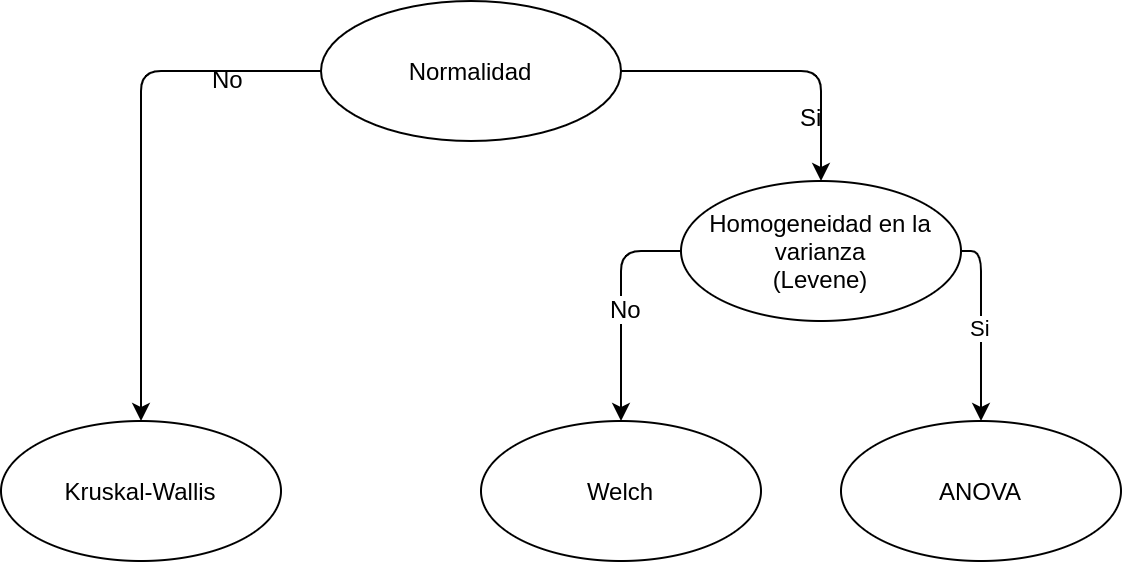
\includegraphics[width=0.8\textwidth]{Tests.png}
\end{tabular}
\centering
\caption{\scriptsize Esquema de las pruebas estadísticas\footcite{Joel:StatisticalTest}.}
\end{figure}

\end{frame}


\section{Convergencia de algoritmos multi-objetivo}


\begin{frame}{Análisis preliminar}
\begin{itemize}
\scriptsize
\justifying
\item Se utilizan los problemas WFG \textit{The Walking Fish Group}.
\justifying
\item Estos problemas dividen a las variables de desición en dos tipos: las variables de distancia y las variables de posición.
\end{itemize}
\begin{figure}
\centering
\begin{tabular}{c}
 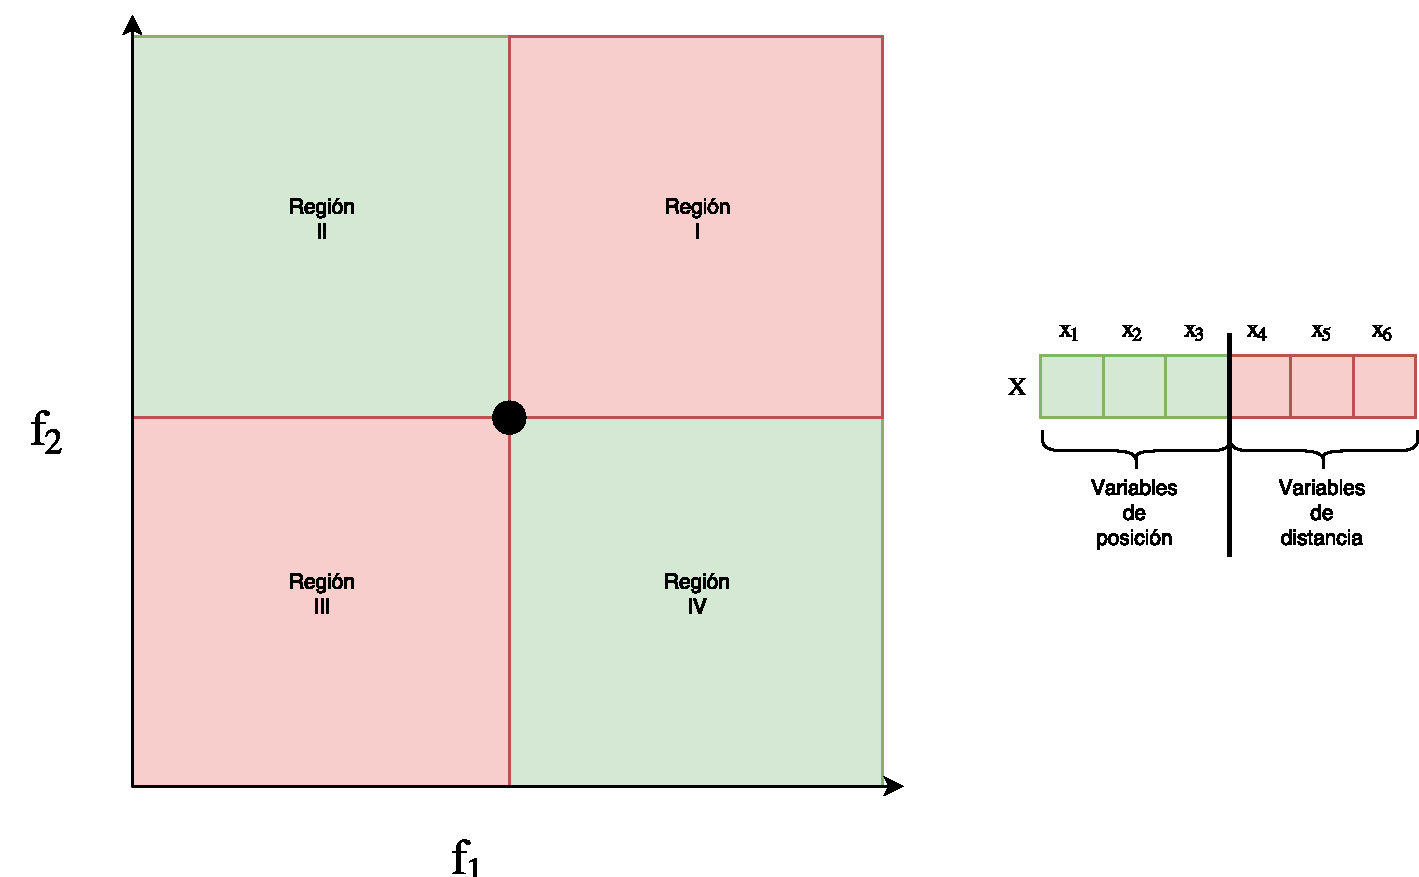
\includegraphics[width=0.9\textwidth]{Parametros_Posicion_Distancia.pdf}   \\
\end{tabular}
\caption{Variables de posición y distancia de los problemas WFG.}
\end{figure}
\end{frame}




\begin{frame}{Análisis preliminar}
\begin{itemize}
\justifying
\item Se eligen los algoritmos NSGA-II, GDE3, MOEA/D y MOMBI-II, siendo basados en dominancia los dos primeros, y basados en descomposición e indicadores los dos últimos.
\justifying
\item Se selecciona el problema de prueba WFG1 que aunque posee una definición simple, muchos MOEAs tienen dificultades de resolverlo.
\justifying
\item Específicamente, la instancia WFG1 es un problema uni-modal y separable.
\justifying
\item La región óptima para el WFG1 esta indicada en la ecuación (\ref{optimo}), donde $k$ es el número de variables de posición y $k+1$ a $n$ son las variables de distancia.
\end{itemize}
\begin{equation} \label{optimo}
	x_{i=k+1:n} = 2i \times 0.35
\end{equation}
\end{frame}

\begin{frame}{Análisis preliminar}
\begin{itemize}
\justifying
\item Se realizaron $35$ ejecuciones con un criterio de paro de $50'000$ generaciones y el tamaño de población de $250$.
\justifying
\item Particularmente, el análisis de diversidad es considerando en las variables de distancia.
\justifying
\item Se calcula la distancia promedio entre los individuos (ADI \textit{Average Distance to all Individuals}).
\end{itemize}
\end{frame}



\begin{frame}{Análisis preliminar}
\begin{itemize}
\justifying
\item En relativamente pocas generaciones (aproximadamente $5'000$), las variables de distancia convergen en todos los métodos.
\justifying
\item En algunas generaciones se recupera la diversidad por el efecto del operador de mutación polinomial.
\end{itemize}

\begin{figure}
\centering
\begin{tabular}{cc}
 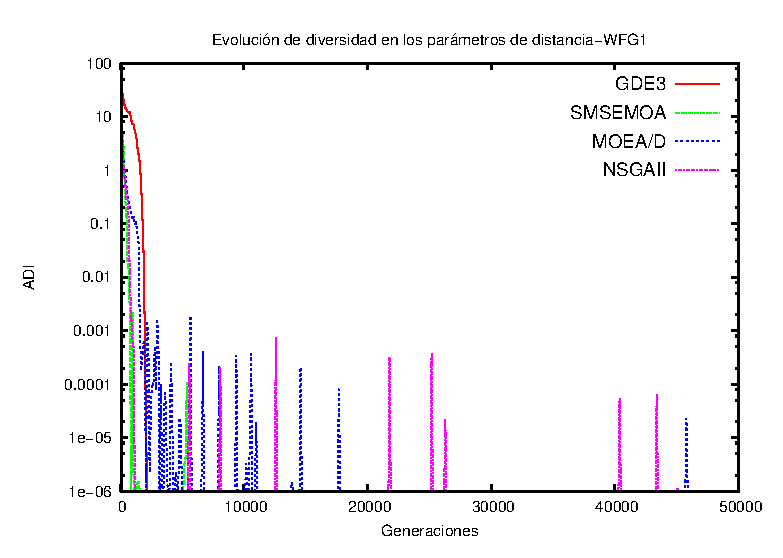
\includegraphics[width=0.5\textwidth]{Average_DistanceParamsStateArt.eps} 
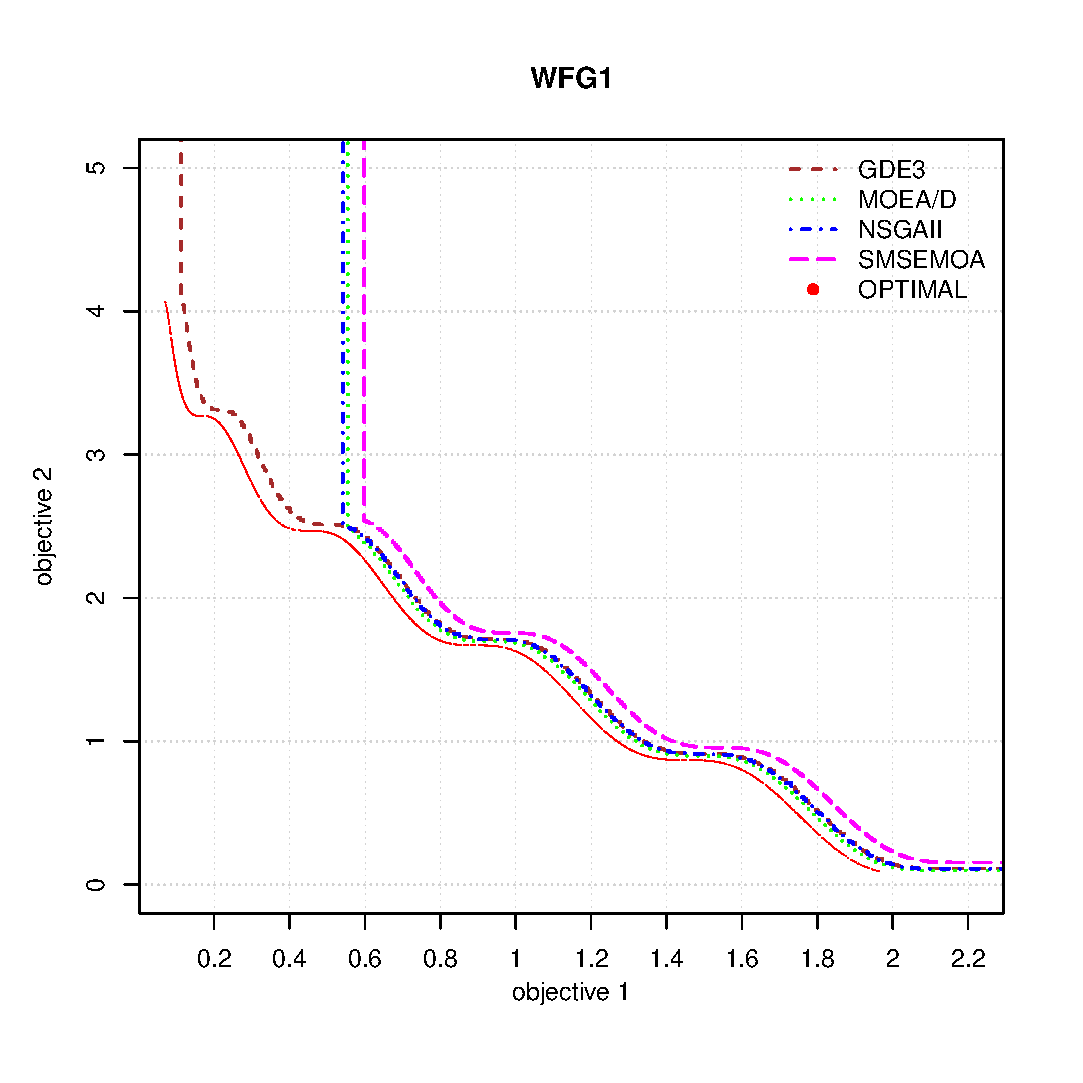
\includegraphics[width=0.35\textwidth]{WFG1_analisis.eps} %\\
\end{tabular}
\caption{Evolución de la diversidad y superficie de alcance al 50\%.}
\label{fig:DiversityProposal}
\end{figure}
\end{frame}


\begin{frame}{Hipótesis}
    \begin{itemize}
        \item Los algoritmos evolutivos tienen un problema de convergencia acelerada en ejecuciones a largo plazo afectando la calidad de las soluciones.
	\item Este problema podría ser tratado implementando mecanismos para administrar la diversidad considerando el tiempo de ejecución y el criterio de parada.
    \end{itemize}
\end{frame}


\section{Algoritmo de diversidad basado en dominancia}

\begin{frame}{Convergencia en el ámbito multi-objetivo}
    \begin{itemize}
        \item Hasta este punto se ha demostrado empíricamente la convergencia prematura en algoritmos multi-objetivo.
	\item A diferencia del caso mono-objetivo, existe muy poco trabajo para administrar la diversidad del espacio de las variables de forma explícita.
	\item Controlar la diversidad en el espacio de las variables puede ser un reto ya que los problemas multi-objetivo podrían mantener diversidad de forma implícita.
	\item ¿Cómo controlar la convergencia en el caso multi-objetivo?
    \end{itemize}
\end{frame}

\begin{frame}{Trabajos relacionados para mantener la diversidad en multi-objetivo}
\begin{itemize}
\scriptsize
    \item Algunos trabajos del área multi-objetivo que consideran la diversidad en el espacio de las variables son los siguientes: \begin{itemize}
	\scriptsize
	\item \citeyear{Joel:NSGA}, NSGA por \citeauthor{Joel:NSGA}.
	\item \citeyear{toffolo2003genetic}, GDEA por \citeauthor{toffolo2003genetic}.
	\item \citeyear{chan2005evolutionary}, KP1, KP2 por \citeauthor{chan2005evolutionary}.
	\item \citeyear{deb2005omni}, Omni-optimizer por \citeauthor{deb2005omni}.
	\item \citeyear{ulrich2010integrating}, DIVA por \citeauthor{ulrich2010integrating}.
    \end{itemize}
   \item Ningún trabajo promueve la diversidad de forma explícita y considera simultáneamente el criterio de parada como en el caso mono-objetivo del trabajo de \textit{Non-Best-Penalized} (BNP) por \citeauthor{romero2018memetic} (\citeyear{romero2018memetic}).
\end{itemize}
\end{frame}



\begin{frame}{Operador de reemplazo \textit{Best-Non-Penalized} BNP}
\begin{algorithm}[H]
\algsetup{linenosize=\tiny}
\caption{BNP Survivor Selection Technique} 
\begin{scriptsize}
\begin{algorithmic}
\STATE Input: $P_t$ (Population of current generation), $Q_t$ (Offspring of current Generation)
   	\STATE Output: $P_{t+1}$ 
        \STATE $R_t = P_t \cup Q_t$ 
        \STATE $P_{t+1} = \emptyset$ 
        \STATE $Penalized = \emptyset$ 
				\STATE $D_t = D_I - D_I * \frac{G_{Elapsed}}{0.5*G_{End}}$
        \WHILE{ $|P_{t+1}|$ $\leq$ N } \label{alg:6}
					\STATE \textcolor{red}{Compute $DCS$ of individuals in $R_t$, using $P_{t+1}$ as a reference set}
					\STATE \textcolor{red}{Move the individuals in $R_t$ with $DCS < D_t$ to $Penalized$}
        	\IF{$R_t$ is empty} \label{alg:9}
						\STATE \textcolor{blue}{ Compute $DCS$ of individuals in $Penalized$, using $P_{t+1}$ as a reference set}
						\STATE \textcolor{blue}{Move the individual in $Penalized$ with the largest $DCS$ to $R_t$}
        	\ENDIF
					\STATE Select the new survivor from $R_t$ as the individual with the best fitness  and move it to $P_{t+1}$
        \ENDWHILE
    	\RETURN $P_{t+1}$ \label{alg:14}
\end{algorithmic}
\end{scriptsize}
\end{algorithm}
\end{frame}



\begin{frame}{Ejemplo}
\begin{figure}[H]
  \centering
  \begin{tabular}{c c}
   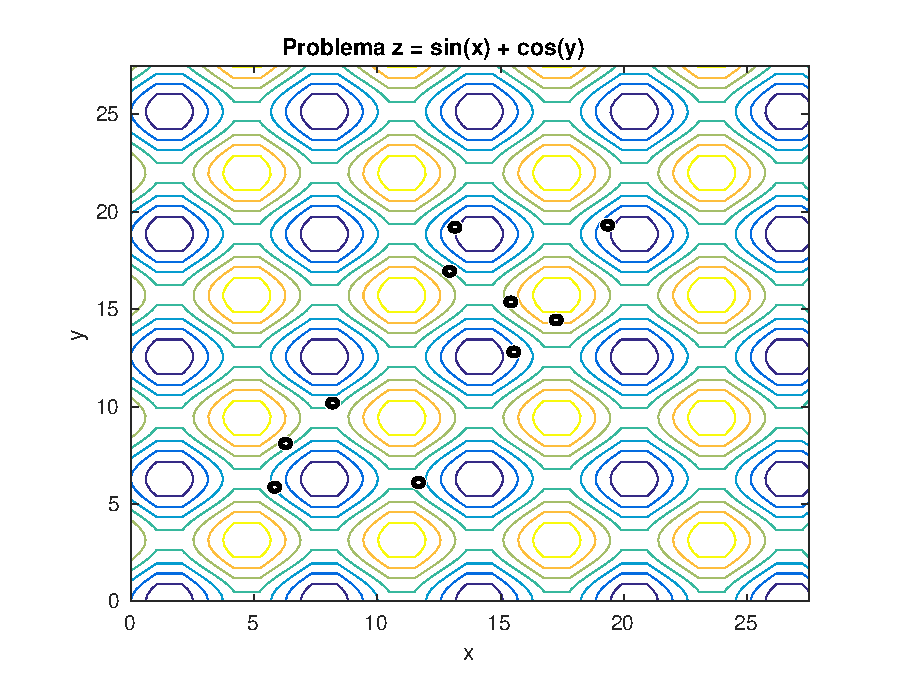
\includegraphics[scale=0.6]{1.eps} 
  \end{tabular}
  \caption{\scriptsize En color negro los candidatos, en rojo los seleccionados y en azul los penalizados.}
\end{figure}
\end{frame}


\begin{frame}{Ejemplo}
\begin{figure}[H]
  \centering
  \begin{tabular}{c c}
   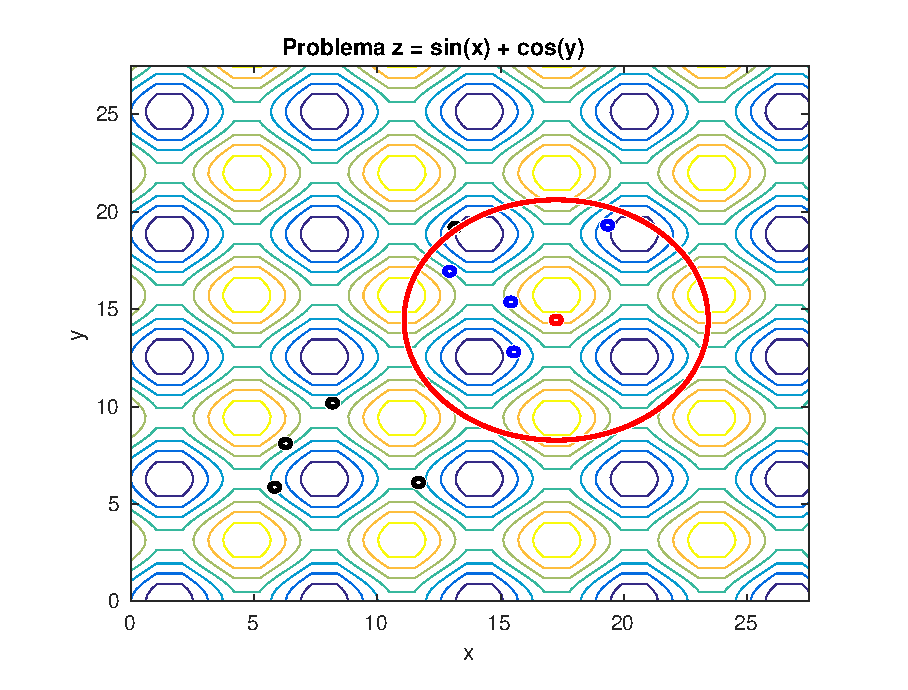
\includegraphics[scale=0.6]{2.eps} 
  \end{tabular}
  \caption{\scriptsize En color negro los candidatos, en rojo los seleccionados y en azul los penalizados.}
\end{figure}
\end{frame}

\begin{frame}{Ejemplo}
\begin{figure}[H]
  \centering
  \begin{tabular}{c c}
   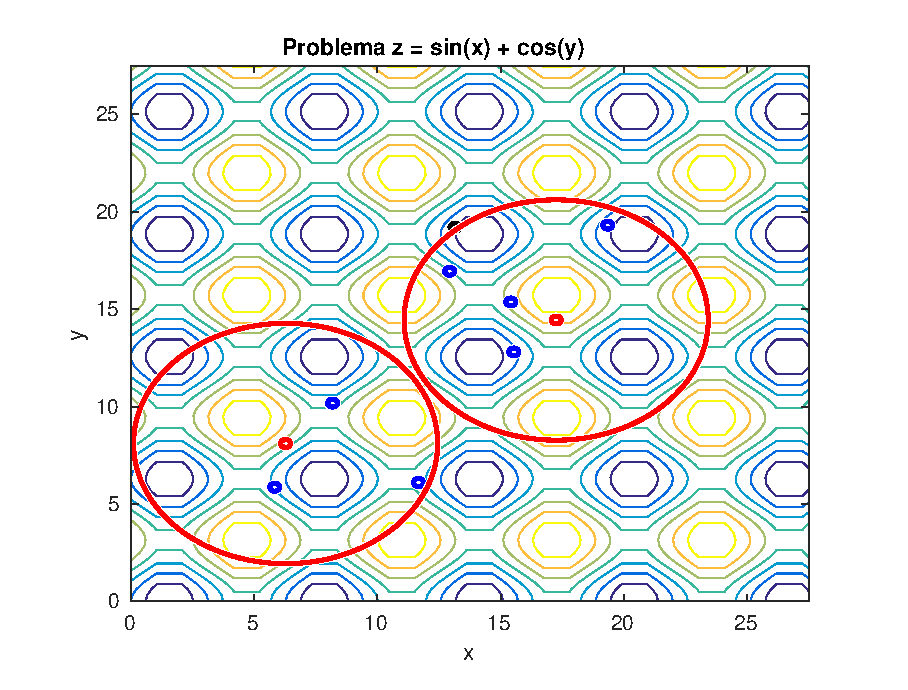
\includegraphics[scale=0.6]{3.eps} 
  \end{tabular}
  \caption{\scriptsize En color negro los candidatos, en rojo los seleccionados y en azul los penalizados.}
\end{figure}
\end{frame}

\begin{frame}{Ejemplo}
\begin{figure}[H]
  \centering
  \begin{tabular}{c c}
   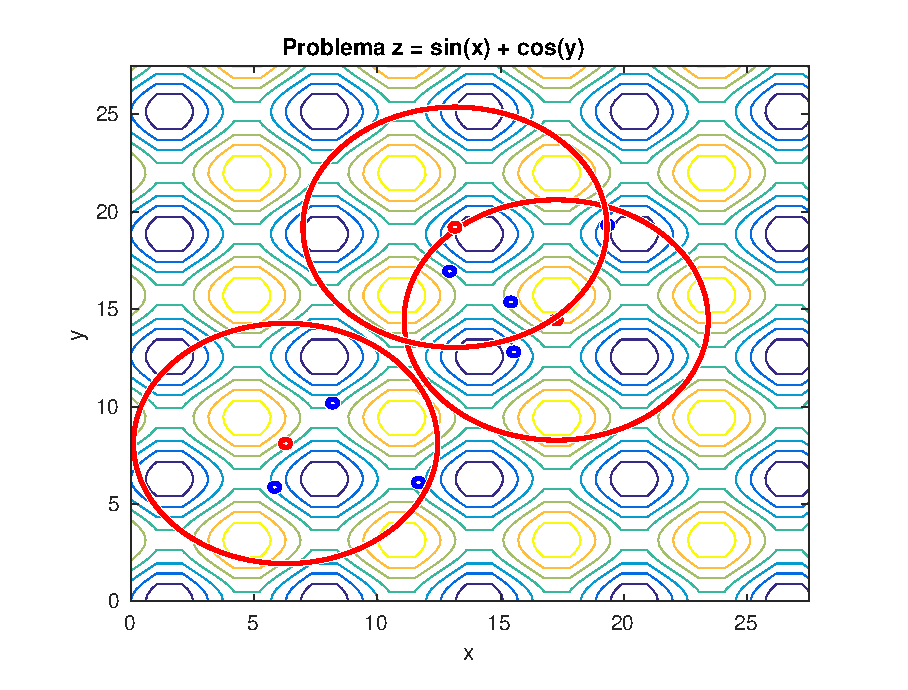
\includegraphics[scale=0.6]{4.eps} 
  \end{tabular}
  \caption{\scriptsize En color negro los candidatos, en rojo los seleccionados y en azul los penalizados.}
\end{figure}
\end{frame}

\begin{frame}{Ejemplo}
\begin{figure}[H]
  \centering
  \begin{tabular}{c c}
   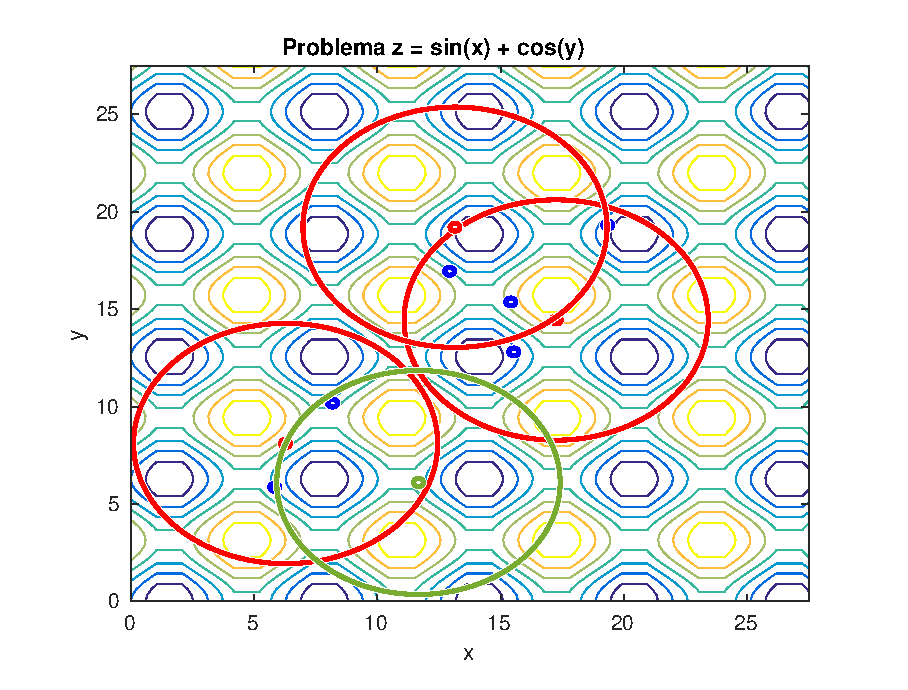
\includegraphics[scale=0.6]{5.eps} 
  \end{tabular}
  \caption{\scriptsize En color negro los candidatos, en rojo los seleccionados y en azul los penalizados.}
\end{figure}
\end{frame}

\begin{frame}{Ejemplo}
\begin{figure}[H]
  \centering
  \begin{tabular}{c c}
   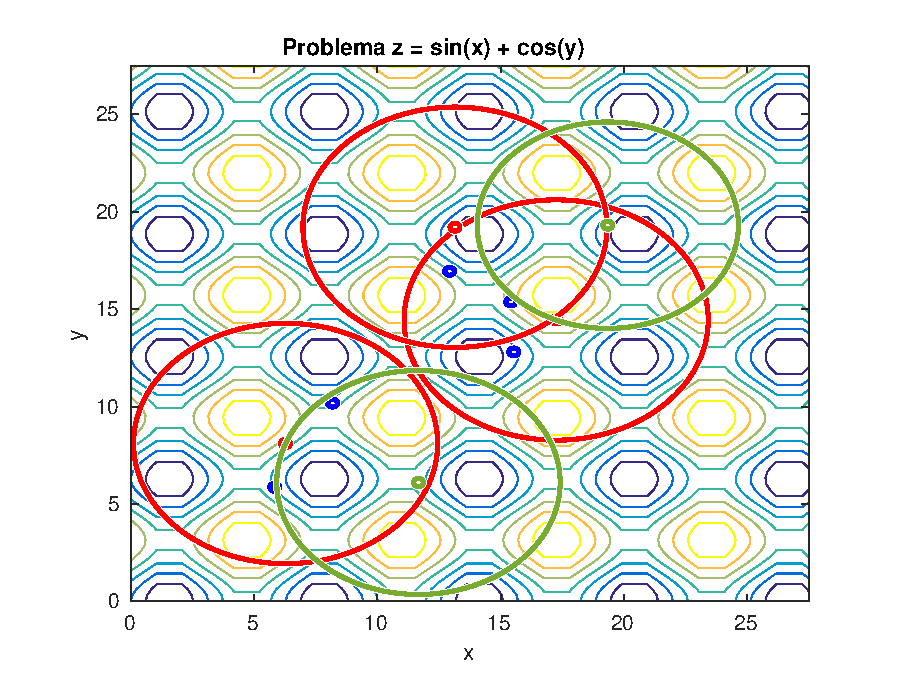
\includegraphics[scale=0.6]{6.eps} 
  \end{tabular}
  \caption{\scriptsize En color negro los candidatos, en rojo los seleccionados y en azul los penalizados.}
\end{figure}
\end{frame}

%\begin{frame}{Ejemplo}
%\begin{figure}[H]
%  \centering
%  \begin{tabular}{c c}
%   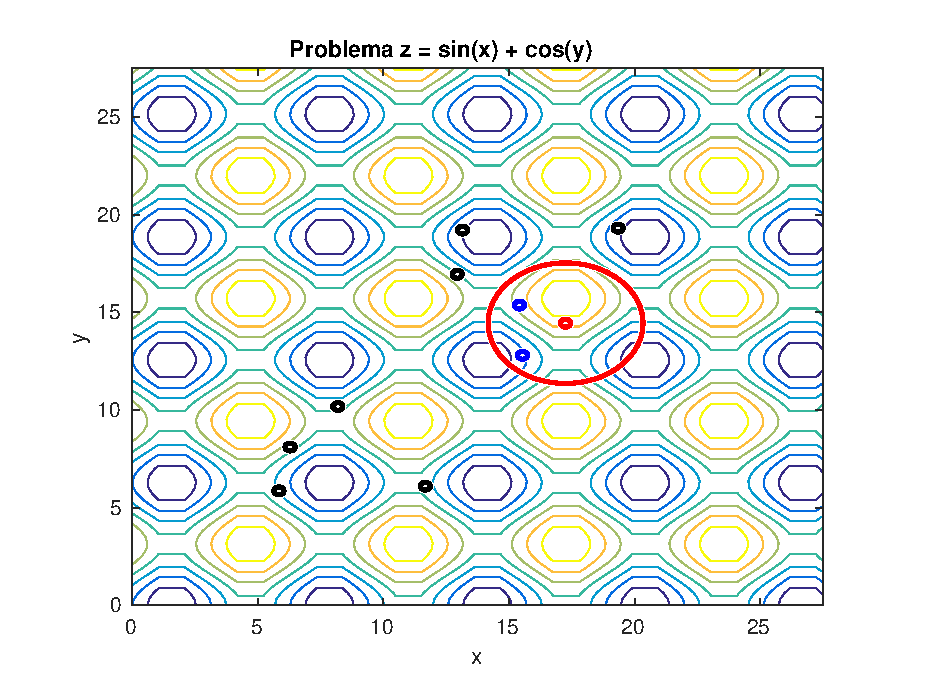
\includegraphics[scale=0.6]{7.eps} 
%  \end{tabular}
%  \caption{\scriptsize En color negro los candidatos, en rojo los seleccionados y en azul los penalizados.}
%\end{figure}
%\end{frame}



\section{Propuesta de diversidad basada en dominancia}

\begin{frame}{Procedimiento principal del VSD-MOEA}
\begin{itemize}
\justifying
\item Se propone al VSD-MOEA (\textit{Variable Space Diversity - Multi-objective Evolutionary Algorithm}).
\justifying
\item Se utiliza el esquema usual de un algoritmo evolutivo.
\justifying
\item Se establece un operador de reemplazo, donde se define un procedimiento para administrar de forma explícita la diversidad.
\end{itemize}
\begin{figure}
\centering
\begin{tabular}{c}
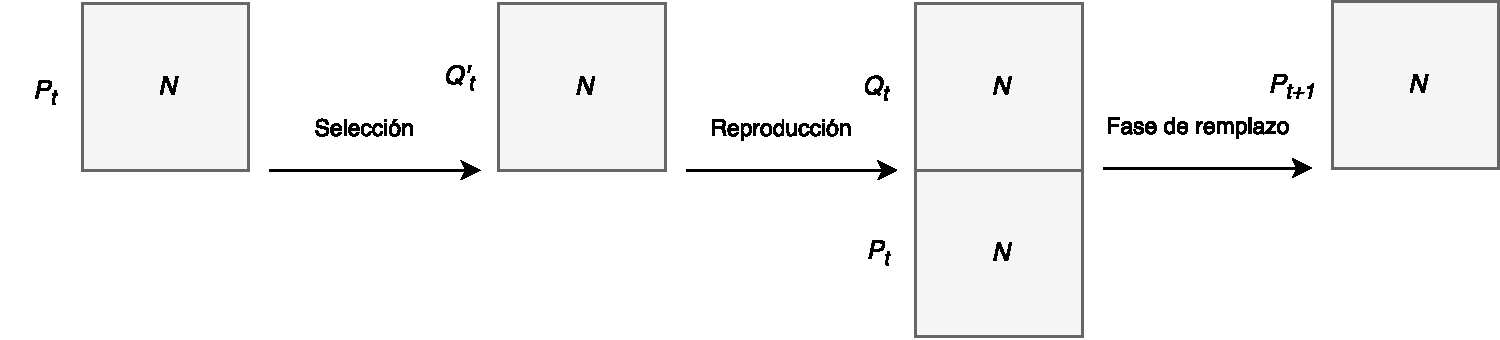
\includegraphics[width=0.9\textwidth]{Evolution_Process.pdf}
\end{tabular}
\caption{Proceso realizado en cada generación.}
\label{fig:DiversityProposal}
\end{figure}
\end{frame}


\begin{frame}{Fase de reemplazo}
\begin{itemize}
\justifying
\item La fase de reemplazo considera un método de penalización.
\justifying
\item El radio de la hiperesfera es decrementado conforme transcurre la ejecución.
\end{itemize}
\begin{figure}
\centering
\begin{tabular}{cc}
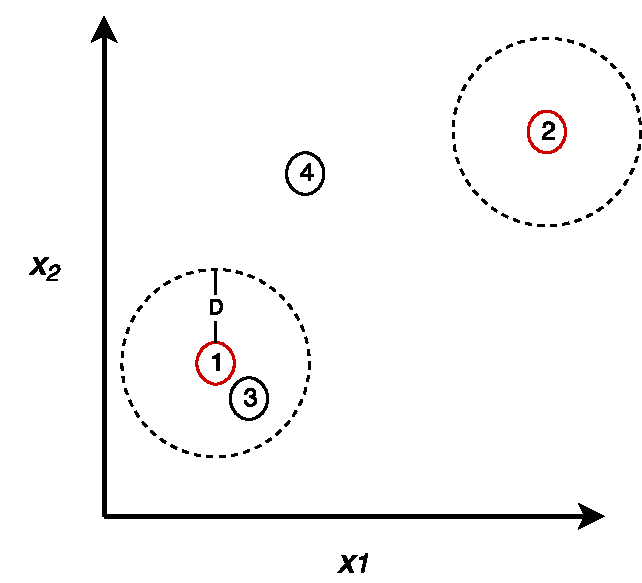
\includegraphics[width=0.35\textwidth]{Metodo_Penalizacion.pdf} \quad \quad \quad
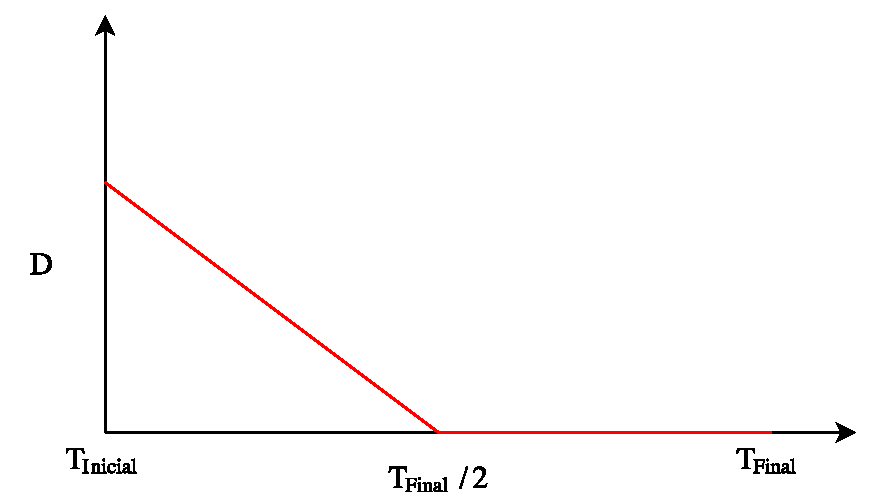
\includegraphics[width=0.6\textwidth]{Modelo.pdf}
\end{tabular}
\label{fig:DiversityProposal}
\end{figure}
\end{frame}



\begin{frame}{Esquema general de la propuesta basada en dominancia}
    \begin{algorithm}[H]
    \begin{scriptsize}
%\algsetup{linenosize=\tiny}
	\caption{Main procedure of VSD-MOEA} 
	\begin{small}
\begin{algorithmic}[1]
 	\STATE \textbf{Initialization}: Generate an initial population $P_0$ with $N$ individuals.
	\STATE \textbf{Evaluation}: Evaluate all individuals in the population.
	\STATE Assign $t=0$
	\WHILE{ (not stopping criterion)  }
	   \STATE \textbf{Mating selection}: Fill the mating pool by performing binary tournament selection on $P_t$, 
		 based on the non-dominated ranks (ties are broken randomly).
	   \STATE \textbf{Variation}: Apply SBX crossover and Polynomial mutation to the mating pool to create a child population $Q_t$.
		 \STATE \textbf{Evaluation}: Evaluate all individuals in $Q_t$.
	   \STATE \textbf{Survivor selecction}: Generate $P_{t+1}$ by applying the replacement scheme 
		 described in Algorithm , using $P_t$ and $Q_t$ as input.
	   \STATE $t=t+1$
	\ENDWHILE
	\end{algorithmic}
	\end{small}
\label{alg:vsd-moea}
\end{scriptsize}
\end{algorithm}
\end{frame}

\begin{frame}{Fase de reemplazo}
Principalmente, la fase de reemplazo se basa en un método de penalización que implementa la métrica de mejoría. \\
($D^b(p_i, r_i) = \sum_{i \in M} max\{0, p_i - r_i\}^2$).
\begin{figure}[t]
\centering




\tikzset{every picture/.style={line width=0.75pt}} %set default line width to 0.75pt        

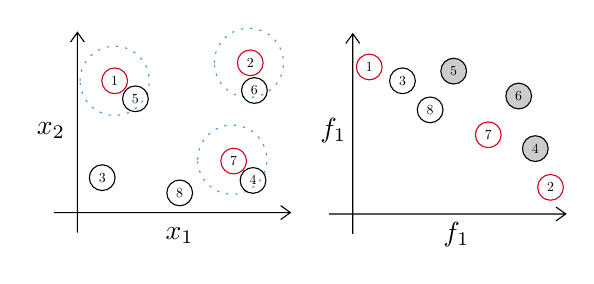
\begin{tikzpicture}[x=0.5pt,y=0.5pt,yscale=-1,xscale=1]
%uncomment if require: \path (0,300); %set diagram left start at 0, and has height of 300

%Shape: Circle [id:dp5136866411017809] 
\draw  [color={rgb, 255:red, 74; green, 144; blue, 226 }  ,draw opacity=1 ][dash pattern={on 0.84pt off 2.51pt}] (69,105) .. controls (69,91.19) and (80.19,80) .. (94,80) .. controls (107.81,80) and (119,91.19) .. (119,105) .. controls (119,118.81) and (107.81,130) .. (94,130) .. controls (80.19,130) and (69,118.81) .. (69,105) -- cycle ;
%Shape: Circle [id:dp3061612047883613] 
\draw  [color={rgb, 255:red, 74; green, 144; blue, 226 }  ,draw opacity=1 ][dash pattern={on 0.84pt off 2.51pt}] (166,92) .. controls (166,78.19) and (177.19,67) .. (191,67) .. controls (204.81,67) and (216,78.19) .. (216,92) .. controls (216,105.81) and (204.81,117) .. (191,117) .. controls (177.19,117) and (166,105.81) .. (166,92) -- cycle ;
%Shape: Axis 2D [id:dp3645341276574614] 
\draw  (50,200.22) -- (221,200.22)(67.1,70) -- (67.1,214.69) (214,195.22) -- (221,200.22) -- (214,205.22) (62.1,77) -- (67.1,70) -- (72.1,77)  ;
%Shape: Circle [id:dp595877391054507] 
\draw  [color={rgb, 255:red, 74; green, 144; blue, 226 }  ,draw opacity=1 ][dash pattern={on 0.84pt off 2.51pt}] (154,162) .. controls (154,148.19) and (165.19,137) .. (179,137) .. controls (192.81,137) and (204,148.19) .. (204,162) .. controls (204,175.81) and (192.81,187) .. (179,187) .. controls (165.19,187) and (154,175.81) .. (154,162) -- cycle ;
%Shape: Axis 2D [id:dp14963900792703488] 
\draw  (249,201.22) -- (420,201.22)(266.1,71) -- (266.1,215.69) (413,196.22) -- (420,201.22) -- (413,206.22) (261.1,78) -- (266.1,71) -- (271.1,78)  ;

% Text Node
\draw  [color={rgb, 255:red, 208; green, 2; blue, 27 }  ,draw opacity=1 ]  (94, 105) circle [x radius= 9.3, y radius= 9.3]   ;
\draw (94,105) node [scale=0.5] [align=left] {1};
% Text Node
\draw  [color={rgb, 255:red, 0; green, 0; blue, 0 }  ,draw opacity=1 ]  (109, 118) circle [x radius= 9.3, y radius= 9.3]   ;
\draw (109,118) node [scale=0.5] [align=left] {5};
% Text Node
\draw  [color={rgb, 255:red, 208; green, 2; blue, 27 }  ,draw opacity=1 ]  (192, 92) circle [x radius= 9.3, y radius= 9.3]   ;
\draw (192,92) node [scale=0.5] [align=left] {2};
% Text Node
\draw    (195, 112) circle [x radius= 9.3, y radius= 9.3]   ;
\draw (195,112) node [scale=0.5] [align=left] {6};
% Text Node
\draw  [color={rgb, 255:red, 208; green, 2; blue, 27 }  ,draw opacity=1 ]  (180, 163) circle [x radius= 9.3, y radius= 9.3]   ;
\draw (180,163) node [scale=0.5] [align=left] {7};
% Text Node
\draw    (194, 177) circle [x radius= 9.3, y radius= 9.3]   ;
\draw (194,177) node [scale=0.5] [align=left] {4};
% Text Node
\draw    (141, 186) circle [x radius= 9.3, y radius= 9.3]   ;
\draw (141,186) node [scale=0.5] [align=left] {8};
% Text Node
\draw    (85, 175) circle [x radius= 9.3, y radius= 9.3]   ;
\draw (85,175) node [scale=0.5] [align=left] {3};
% Text Node
\draw  [color={rgb, 255:red, 208; green, 2; blue, 27 }  ,draw opacity=1 ]  (278, 95) circle [x radius= 9.3, y radius= 9.3]   ;
\draw (278,95) node [scale=0.5] [align=left] {1};
% Text Node
\draw  [color={rgb, 255:red, 0; green, 0; blue, 0 }  ,draw opacity=1 ][fill={rgb, 255:red, 0; green, 0; blue, 0 }  ,fill opacity=0.2 ]  (339, 98) circle [x radius= 9.3, y radius= 9.3]   ;
\draw (339,98) node [scale=0.5] [align=left] {5};
% Text Node
\draw  [color={rgb, 255:red, 208; green, 2; blue, 27 }  ,draw opacity=1 ]  (409, 182) circle [x radius= 9.3, y radius= 9.3]   ;
\draw (409,182) node [scale=0.5] [align=left] {2};
% Text Node
\draw  [fill={rgb, 255:red, 0; green, 0; blue, 0 }  ,fill opacity=0.2 ]  (386, 116) circle [x radius= 9.3, y radius= 9.3]   ;
\draw (386,116) node [scale=0.5] [align=left] {6};
% Text Node
\draw  [color={rgb, 255:red, 208; green, 2; blue, 27 }  ,draw opacity=1 ]  (364, 144) circle [x radius= 9.3, y radius= 9.3]   ;
\draw (364,144) node [scale=0.5] [align=left] {7};
% Text Node
\draw  [fill={rgb, 255:red, 0; green, 0; blue, 0 }  ,fill opacity=0.2 ]  (398, 154) circle [x radius= 9.3, y radius= 9.3]   ;
\draw (398,154) node [scale=0.5] [align=left] {4};
% Text Node
\draw    (322, 126) circle [x radius= 9.3, y radius= 9.3]   ;
\draw (322,126) node [scale=0.5] [align=left] {8};
% Text Node
\draw    (302, 105) circle [x radius= 9.3, y radius= 9.3]   ;
\draw (302,105) node [scale=0.5] [align=left] {3};
% Text Node
\draw (141,217) node   {$x_{1}$};
% Text Node
\draw (48,141) node   {$x_{2}$};
% Text Node
\draw (341,216) node   {$f_{1}$};
% Text Node
\draw (252,141) node   {$f_{1}$};


\end{tikzpicture}


%\includegraphics[width=0.45\textwidth]{Images/Fase_Remplazo_2.eps}
\caption{Método de penalización de la fase de reemplazo.} \label{fig:Hypersphere}
\end{figure}
\end{frame}

\begin{frame}{Fase de reemplazo}
  \begin{algorithm}[H]
  \begin{scriptsize}
%\algsetup{linenosize=\tiny}
	\caption{Replacement Phase of VSD-MOEA} 
\begin{algorithmic}[1]
\STATE Input: $P_t$ (Population of current generation), $Q_t$ (Offspring of current Generation)
    	\STATE Output: $P_{t+1}$ 
        \STATE $R_t = P_t \cup Q_t$ \label{alg:1}
        \STATE $P_{t+1} = \emptyset$ \label{alg:2}
        \STATE $Penalized = \emptyset$ \label{alg:3}
				\STATE $D_t = D_I - D_I * \frac{G_{Elapsed}}{0.9*G_{End}}$ \label{alg:4}
%				\FOR{$k \in {1...M}$}\label{alg:5}
%					\STATE Move to $P_{t+1}$ the individual that optimize $AWF_k$ (Eq.~\ref{eqn:extremes}) \label{alg:5b}
%				\ENDFOR
        \WHILE{ $|P_{t+1}|$ $\leq$ N } \label{alg:6}
					\STATE Compute $DCS$ of individuals in $R_t$ with $P_{t+1}$ used as reference set \label{alg:7}
					\STATE Move to $Penalized$ the individuals in $R_t$ with $DCS < D_t$  \label{alg:8}
        	\IF{$R_t$ is empty} \label{alg:9}
						\STATE Compute $DCS$ of individuals in $Penalized$ with $P_{t+1}$ used as reference set \label{alg:10}
						\STATE Move to $R_t$ the individual in $Penalized$ with largest $DCS$ \label{alg:11}
        	\ENDIF
					\STATE Identify the first front ($F$) in $R_t \cup P_{t+1}$ with an individual $I \in R_t$ \label{alg:12}
					\STATE Use the novel density estimator  to select a new survivor 
					from $F$ and move it to $P_{t+1}$\label{alg:13}
        \ENDWHILE
    	\RETURN $P_{t+1}$ \label{alg:14}
	\end{algorithmic}

\label{alg:Replacement_Phase}
\end{scriptsize}
\end{algorithm}
\end{frame}




\begin{frame}{Procedimiento de selección}
El estimador de densidad en el espacio objetivo considera el indicador ASF y la distancia de mejoría.
\begin{equation}\label{eqn:extremes}
\scriptsize
AWF_k (\vec{x}) = f_k(\vec{x}) + 10^{-4} \times  \sum_{j=1}^M f_j( \vec{x} )
\end{equation}

%\begin{itemize}
%\justifying
%\item Seleccionar al individuo con la mayor distancia al vecino de re\-fe\-ren\-cia más cercano, puede causar selecciones no deseables, como se puede observar en la siguiente imágen.
%\end{itemize}
\begin{figure}[H]
\centering
\scriptsize
\includegraphics[scale=0.35]
{Atipico.pdf}
%\caption{ Análisis del procedimiento de selección propuesto, las soluciones de referencia están representadas con bordes de color rojo, las soluciones candidatas con bordes de color verde, el frente de Pareto está representado por una línea roja punteada.}
\label{fig:Atipico}
\end{figure}
\end{frame}

\begin{frame}{Procedimiento de selección}
\begin{algorithm}[H]
\algsetup{linenosize=\tiny}
	\caption{Density estimator} 
\begin{scriptsize}
\begin{algorithmic}
\STATE Input: $P_{t+1}$ (Survivors), $R_t$ (Candidates), $F$ (Current front)
    	\STATE Output: $I \in R_t$ 
	\STATE $FP = P_{t+1} \cap F$ \label{alg:FP}
	\STATE $FR = R_{t} \cap F$ \label{alg:FR}
        \FOR{$k \in$ number of objectives}\label{alg:density_for}
	      \STATE Select the best individual $I \in F$ of $k$ according to Eq.~\ref{eqn:extremes}.\label{alg:density_1}
	  	\IF{ $I \in FR$}
	  	 \RETURN $I$ \label{alg:density_2}
	  	\ENDIF
	\ENDFOR\label{alg:density_endfor}
	\STATE $MaxID = 0$ \label{alg:density_for2}
	\FOR{ $ Ic \in FR$}
	\STATE $Improvement = \displaystyle{\min_{s \in FP}\ ID(Ic, s)}$ 
	\IF{ $Improvement > MaxID$} \label{alg:density_if2}
	   \STATE $MaxID = Improvement$
	   \STATE $I = Ic$ 
	\ENDIF \label{alg:density_endif2}
	\ENDFOR	\label{alg:density_endfor2}
    	\RETURN $I$ \label{alg:density_4}
	\end{algorithmic}
\end{scriptsize}
\end{algorithm}
\end{frame}


\begin{frame}{Comparación del estado-del-arte con ejecuciones a largo plazo}
\begin{itemize}
\scriptsize
\item Se consideran $250'000$ generaciones.
\item Se considera el MOEA/D, NSGA-II y R2-EMOA.
\item Los problemas que se consideraron fueron DTLZ, WFG y UF.
\end{itemize}

% Please add the following required packages to your document preamble:
% \usepackage{graphicx}
\begin{table}[t]
\centering
\caption{Statistical Tests and Deterioration Level of the \HV{} ratio for problems with two objectives}
\label{tab:Tests_HV_2obj}

%\resizebox{\textwidth}{!}{%
\begin{scriptsize}
\begin{tabular}{c c|c|c|c}
\cline{2-5}
                                        & \textbf{$\uparrow$} & \textbf{$\downarrow$} & \textbf{$\leftrightarrow$} & \textbf{Deterioration} \\ \hline
\multicolumn{1}{c|}{\textbf{MOEA/D}}   & 24                  & 36                    & 9                          & 1.615         \\ \hline
\multicolumn{1}{c|}{\textbf{NSGA-II}}  & 13                  & 49                    & 7                          & 1.496         \\ \hline
\multicolumn{1}{c|}{\textbf{R2-EMOA}}  & 34                  & 21                    & 14                         & 1.597         \\ \hline
\multicolumn{1}{c|}{\textbf{VSD-MOEA}} & 50                  & 15                    & 4                          & 0.059         \\ \hline
\end{tabular}%
\end{scriptsize}
%}
\end{table}


%

% Please add the following required packages to your document preamble:
% \usepackage{graphicx}
\begin{table}[t]
\caption{\scriptsize Statistical Tests and Deterioration Level of the \HV{} ratio for problems with three objectives}
\label{tab:Tests_HV_3obj}
\centering
%\resizebox{\textwidth}{!}{%
\begin{scriptsize}
\begin{tabular}{c c|c|c|c}
\cline{2-5}
                                        & \textbf{$\uparrow$} & \textbf{$\downarrow$} & \textbf{$\leftrightarrow$} & \textbf{Deterioration} \\ \hline
\multicolumn{1}{c|}{\textbf{MOEA/D}}   & 16                  & 37                    & 4                          & 1.601         \\ \hline
\multicolumn{1}{c|}{\textbf{NSGA-II}}  & 9                   & 45                    & 3                          & 2.557         \\ \hline
\multicolumn{1}{c|}{\textbf{R2-EMOA}}  & 31                  & 22                    & 4                          & 1.223         \\ \hline
\multicolumn{1}{c|}{\textbf{VSD-MOEA}} & 52                  & 4                     & 1                          & 0.037         \\ \hline
\end{tabular}%
\end{scriptsize}
%}
\end{table}
%

\end{frame}

\begin{frame}{Comparación del estado-del-arte con ejecuciones a largo plazo}
% Please add the following required packages to your document preamble:
% \usepackage{graphicx}
\begin{table}[t]
\caption{Summary of the hypervolume ratio results attained for problems with two objectives}
\centering
\begin{scriptsize}
\resizebox{\textwidth}{!}{%
\begin{tabular}{cc|c|c|c|c|c|c|c|c|c|c|c|c|c|c|c}
\cline{2-17}
\textbf{}                           & \multicolumn{4}{c|}{\textbf{MOEA/D}}                              & \multicolumn{4}{c|}{\textbf{NSGA-II}}                             & \multicolumn{4}{c|}{\textbf{R2-EMOA}}                             & \multicolumn{4}{c}{\textbf{VSD-MOEA}}                            \\ \cline{2-17} 
                                    & \textbf{Min}   & \textbf{Max}   & \textbf{Mean}  & \textbf{Std}   & \textbf{Min}   & \textbf{Max}   & \textbf{Mean}  & \textbf{Std}   & \textbf{Min}   & \textbf{Max}   & \textbf{Mean}  & \textbf{Std}   & \textbf{Min}   & \textbf{Max}   & \textbf{Mean}  & \textbf{Std}   \\ \hline
\multicolumn{1}{c|}{\textbf{WFG1}}  & \textbf{0.984} & \textbf{0.993} & \textbf{0.992} & \textbf{0.002} & 0.987          & 0.993          & 0.992          & 0.002          & 0.946          & 0.994          & 0.988          & 0.012          & 0.980          & 0.994          & 0.992          & 0.003          \\ \hline
\multicolumn{1}{c|}{\textbf{WFG2}}  & 0.965          & 0.996          & 0.967          & 0.007          & 0.966          & 0.998          & 0.974          & 0.014          & 0.965          & 0.966          & 0.966          & 0.000          & \textbf{0.998} & \textbf{0.998} & \textbf{0.998} & \textbf{0.000} \\ \hline
\multicolumn{1}{c|}{\textbf{WFG3}}  & 0.992          & 0.992          & 0.992          & 0.000          & 0.987          & 0.988          & 0.987          & 0.000          & 0.991          & 0.992          & 0.991          & 0.000          & \textbf{0.992} & \textbf{0.992} & \textbf{0.992} & \textbf{0.000} \\ \hline
\multicolumn{1}{c|}{\textbf{WFG4}}  & 0.988          & 0.988          & 0.988          & 0.000          & 0.983          & 0.987          & 0.985          & 0.001          & \textbf{0.991} & \textbf{0.991} & \textbf{0.991} & \textbf{0.000} & 0.990          & 0.990          & 0.990          & 0.000          \\ \hline
\multicolumn{1}{c|}{\textbf{WFG5}}  & 0.876          & 0.893          & 0.882          & 0.005          & 0.884          & 0.899          & 0.890          & 0.002          & 0.886          & 0.895          & 0.891          & 0.003          & \textbf{0.894} & \textbf{0.928} & \textbf{0.914} & \textbf{0.010} \\ \hline
\multicolumn{1}{c|}{\textbf{WFG6}}  & \textbf{0.879} & \textbf{0.940} & \textbf{0.914} & \textbf{0.016} & \textbf{0.894} & \textbf{0.942} & \textbf{0.913} & \textbf{0.012} & \textbf{0.875} & \textbf{0.942} & \textbf{0.912} & \textbf{0.015} & 0.855          & 0.888          & 0.868          & 0.007          \\ \hline
\multicolumn{1}{c|}{\textbf{WFG7}}  & 0.988          & 0.988          & 0.988          & 0.000          & 0.983          & 0.987          & 0.984          & 0.001          & \textbf{0.991} & \textbf{0.991} & \textbf{0.991} & \textbf{0.000} & 0.990          & 0.990          & 0.990          & 0.000          \\ \hline
\multicolumn{1}{c|}{\textbf{WFG8}}  & 0.800          & 0.822          & 0.811          & 0.006          & 0.771          & 0.801          & 0.789          & 0.006          & 0.803          & 0.824          & 0.815          & 0.005          & \textbf{0.828} & \textbf{0.958} & \textbf{0.928} & \textbf{0.046} \\ \hline
\multicolumn{1}{c|}{\textbf{WFG9}}  & 0.795          & 0.972          & 0.883          & 0.082          & 0.793          & 0.966          & 0.832          & 0.070          & 0.797          & 0.976          & 0.884          & 0.079          & \textbf{0.963} & \textbf{0.975} & \textbf{0.970} & \textbf{0.004} \\ \hline
\multicolumn{1}{c|}{\textbf{DTLZ1}} & \textbf{0.993} & \textbf{0.993} & \textbf{0.993} & \textbf{0.000} & 0.990          & 0.992          & 0.991          & 0.000          & 0.992          & 0.992          & 0.992          & 0.000          & 0.992          & 0.992          & 0.992          & 0.000          \\ \hline
\multicolumn{1}{c|}{\textbf{DTLZ2}} & 0.989          & 0.989          & 0.989          & 0.000          & 0.986          & 0.988          & 0.987          & 0.000          & \textbf{0.991} & \textbf{0.992} & \textbf{0.992} & \textbf{0.000} & 0.990          & 0.990          & 0.990          & 0.000          \\ \hline
\multicolumn{1}{c|}{\textbf{DTLZ3}} & 0.989          & 0.989          & 0.989          & 0.000          & 0.987          & 0.989          & 0.989          & 0.001          & \textbf{0.991} & \textbf{0.992} & \textbf{0.992} & \textbf{0.000} & 0.990          & 0.990          & 0.990          & 0.000          \\ \hline
\multicolumn{1}{c|}{\textbf{DTLZ4}} & 0.259          & 0.989          & 0.781          & 0.330          & 0.259          & 0.988          & 0.863          & 0.274          & 0.259          & 0.992          & 0.657          & 0.365          & \textbf{0.990} & \textbf{0.990} & \textbf{0.990} & \textbf{0.000} \\ \hline
\multicolumn{1}{c|}{\textbf{DTLZ5}} & 0.989          & 0.989          & 0.989          & 0.000          & 0.986          & 0.988          & 0.987          & 0.000          & \textbf{0.991} & \textbf{0.992} & \textbf{0.992} & \textbf{0.000} & 0.990          & 0.990          & 0.990          & 0.000          \\ \hline
\multicolumn{1}{c|}{\textbf{DTLZ6}} & 0.448          & 0.910          & 0.700          & 0.105          & 0.138          & 0.511          & 0.322          & 0.075          & 0.510          & 0.922          & 0.691          & 0.107          & \textbf{0.990} & \textbf{0.990} & \textbf{0.990} & \textbf{0.000} \\ \hline
\multicolumn{1}{c|}{\textbf{DTLZ7}} & 0.996          & 0.996          & 0.996          & 0.000          & 0.996          & 0.997          & 0.996          & 0.000          & \textbf{0.997} & \textbf{0.997} & \textbf{0.997} & \textbf{0.000} & 0.996          & 0.996          & 0.996          & 0.000          \\ \hline
\multicolumn{1}{c|}{\textbf{UF1}}   & 0.991          & 0.993          & 0.992          & 0.000          & 0.986          & 0.989          & 0.988          & 0.000          & 0.978          & 0.994          & 0.990          & 0.005          & \textbf{0.994} & \textbf{0.995} & \textbf{0.994} & \textbf{0.000} \\ \hline
\multicolumn{1}{c|}{\textbf{UF2}}   & \textbf{0.987} & \textbf{0.993} & \textbf{0.991} & \textbf{0.002} & 0.980          & 0.983          & 0.981          & 0.001          & 0.984          & 0.991          & 0.988          & 0.002          & 0.987          & 0.993          & 0.990          & 0.001          \\ \hline
\multicolumn{1}{c|}{\textbf{UF3}}   & 0.481 	     & 0.674 	      & 0.597          & 0.043          & 0.678          & 0.871          & 0.784          & 0.048          & 0.531          & 0.704          & 0.589          & 0.041          & \textbf{0.799} & \textbf{0.916} & \textbf{0.881} & \textbf{0.025} \\ \hline
\multicolumn{1}{c|}{\textbf{UF4}}   & 0.881          & 0.917          & 0.908          & 0.006          & 0.875          & 0.910          & 0.889          & 0.008          & \textbf{0.923} & \textbf{0.935} & \textbf{0.929} & \textbf{0.003} & 0.923          & 0.931          & 0.927          & 0.002          \\ \hline
\multicolumn{1}{c|}{\textbf{UF5}}   & 0.035          & 0.792          & 0.484          & 0.165          & 0.256          & 0.766          & 0.641          & 0.104          & 0.123          & 0.792          & 0.566          & 0.192          & \textbf{0.582} & \textbf{0.763} & \textbf{0.647} & \textbf{0.040} \\ \hline
\multicolumn{1}{c|}{\textbf{UF6}}   & 0.255          & 0.711          & 0.447          & 0.114          & 0.235          & 0.801          & 0.635          & 0.120          & 0.349          & 0.767          & 0.568          & 0.113          & \textbf{0.668} & \textbf{0.900} & \textbf{0.810} & \textbf{0.061} \\ \hline
\multicolumn{1}{c|}{\textbf{UF7}}   & \textbf{0.987} & \textbf{0.991} & \textbf{0.990} & \textbf{0.001} & 0.980          & 0.983          & 0.981          & 0.001          & 0.557          & 0.991          & 0.910          & 0.150          & \textbf{0.975} & \textbf{0.992} & \textbf{0.988} & \textbf{0.004} \\ \hline
\multicolumn{1}{c|}{\textbf{Mean}}  & 0.806          & 0.935          & 0.881          & 0.038          & 0.808          & 0.927          & 0.886          & 0.032          & 0.801          & 0.940          & 0.882          & 0.048          & 0.929          & 0.963          & 0.949          & 0.009          \\ \hline
\end{tabular}%
}
\end{scriptsize}
\end{table}


\end{frame}




%\begin{frame}{Superficies de cubrimiento}
%Poner superficie de diferencias.
%\end{frame}

\begin{frame}{Análisis de escalabilidad en el espacio de las variables}
\begin{itemize}
\item Se hizo un análisis de escalabilidad con 50, 100 y 250 variables, considerando $25'000$ generaciones.
\end{itemize}
\begin{figure}
\centering
\begin{tabular}{cc}
\includegraphics[scale=0.6]{Images/Graphic-Scalability-2obj_tikz-figure0.eps} & \includegraphics[scale=0.6]{Images/Graphic-Scalability-3obj_tikz-figure0.eps}
\end{tabular}
\caption{Mean of the \HV{} ratio for 35 runs for the two-objective and three-objective problems considering different numbers of variables}
\end{figure}
\end{frame}

\begin{frame}{Análisis de diversidad en el espacio de la variables}
\begin{itemize}
\item Se observa que el VSD-MOEA mantiene un grado de diversidad en los parámetros de distancia en los problemas WFG.
\end{itemize}
\begin{figure}
\centering
\begin{tabular}{cc}
\includegraphics[scale=0.6]{Images/Graphic-Diversity_2obj_tikz-figure1.eps} & \includegraphics[scale=0.6]{Images/Graphic-Diversity_3obj_tikz-figure1.eps} 
\end{tabular}
\caption{Evolution of ADI for problems WFG1-WFG7 with two objectives considering only the distance variables}
\end{figure}
\end{frame}


\begin{frame}{Análisis de rendimiento en función al criterio de paro}
\begin{figure}[t]
\centering
\begin{tabular}{l}
 \includegraphics[scale=0.6]{Images/Time_tikz-figure0.eps}\\[0cm]%[-0.14cm] 
 \includegraphics[scale=0.6]{Images/Time_tikz-figure1.eps}\\[0cm]%[-0.18cm]
 \includegraphics[scale=0.6]{Images/Time_tikz-figure2.eps}
\end{tabular}
\caption{\scriptsize Performance of MOEAs for the problems with two objectives considering three ranges for the stopping criterion: 
short-term (first row), middle-term (second row) and long-term (third row).}
\end{figure}
\end{frame}

\begin{frame}{Análisis de rendimiento en función al criterio de paro}
\begin{figure}[t]
\centering
\begin{tabular}{l}
 \includegraphics[scale=0.6]{Images/Time_tikz-figure3.eps}\\[0cm]%[-0.14cm] 
 \includegraphics[scale=0.6]{Images/Time_tikz-figure4.eps}\\[0cm]%[-0.18cm]
 \includegraphics[scale=0.6]{Images/Time_tikz-figure5.eps}
\end{tabular}
\caption{\scriptsize Performance of MOEAs for the problems with three objectives considering three ranges for the stopping 
criterion: short-term (first row), middle-term (second row) and long-term (third row).}
\end{figure}
\end{frame}




\begin{frame}{Análisis del umbral de diversidad inicial}
\begin{itemize}
\item Se hizo un análisis del parámetro que induce el grado de diversidad inicial en el operador de reemplazo.
\item El mejor valor en dos como en tres objetivos es de $0.4$.
\end{itemize}
\begin{figure}[t]
\centering
\includegraphics[scale=0.85]{Images/Graphic-Initial-Distance_tikz-figure0.eps} \\
\caption{Mean of \HV{} values taking into account all the problems with several initial threshold values}\label{fig:Initial-distance-factor}
\end{figure}
\end{frame}

\begin{frame}{Simulación}
\begin{itemize}
\scriptsize
\justifying
\item Se realiza una simulación con el problema WFG5.
\item Se configuró el problema WFG5 con dos variables de decisión, una variable de posición y una variable de distancia.
\item En esta configuración el conjunto de Pareto está definido en $x_2 = 1.4$
\item Este problema está compuesto por funciones con características deceptivas.
\end{itemize}
\begin{figure}[t]
\centering
\includegraphics[scale=0.2]{deceptiva_wfg5.png} \\
%\caption{Mean of \HV{} values taking into account all the problems with several initial threshold values}\label{fig:Initial-distance-factor}
\end{figure}
\centering
\url{https://youtu.be/dbk5DaFJ8y0}
\end{frame}

\begin{frame}{Trabajo en progreso}
\begin{itemize}
\scriptsize
    \item Con el mismo principio se está desarrollando el algortimos multi-objetivo basado en descomposición.
    \item En este caso se consideran los operadores de evolución diferencial.
\end{itemize}
\begin{figure}
\centering
\begin{tabular}{cc}
\includegraphics[scale=0.4]{general_mean_HV.eps} 
\end{tabular}
%\caption{Evolution of ADI for problems WFG1-WFG7 with two objectives considering only the distance variables}
\end{figure}
\end{frame}

\begin{frame}{Trabajo en progreso}
\begin{itemize}
    \item La versión basada en descomposición es mejor que la de dominancia en dos objetivos.
\end{itemize}
\begin{figure}
\centering
\begin{tabular}{cc}
\includegraphics[scale=0.4]{factor_inicial.eps} 
\end{tabular}
%\caption{Evolution of ADI for problems WFG1-WFG7 with two objectives considering only the distance variables}
\end{figure}

\end{frame}




\section{Conclusiones y trabajo futuro}
\begin{frame}{Conclusiones y trabajo futuro}
    \begin{itemize}
        \item Los algoritmos evolutivos que consideran la diversidad en el espacio de las variables de forma explícita y en función al criterio de parada ofrecen soluciones de calidad en esquemas de largo plazo. 
        \item En el caso multi-objetivo, la cantidad de evaluaciones a función necesarias para mejorar al estado del arte es a partir de 2'500 generaciones.
        \item Con el fin de obtener un rendimiento superior en los algoritmos de optimización es necesario considerar el criterio de parada para tomar decisiones.
    \end{itemize}
\end{frame}




%\begin{frame}{Acknowledgements}
%Este ta
%This work has been supported by the Center for Research in Mathematics.
%\end{frame}

\end{document}
